\documentclass[twoside]{book}

% Packages required by doxygen
\usepackage{calc}
\usepackage{doxygen}
\usepackage{graphicx}
\usepackage[utf8]{inputenc}
\usepackage{makeidx}
\usepackage{multicol}
\usepackage{multirow}
\usepackage{textcomp}
\usepackage[table]{xcolor}

% Font selection
\usepackage[T1]{fontenc}
\usepackage{mathptmx}
\usepackage[scaled=.90]{helvet}
\usepackage{courier}
\usepackage{amssymb}
\usepackage{sectsty}
\renewcommand{\familydefault}{\sfdefault}
\allsectionsfont{%
  \fontseries{bc}\selectfont%
  \color{darkgray}%
}
\renewcommand{\DoxyLabelFont}{%
  \fontseries{bc}\selectfont%
  \color{darkgray}%
}

% Page & text layout
\usepackage{geometry}
\geometry{%
  a4paper,%
  top=2.5cm,%
  bottom=2.5cm,%
  left=2.5cm,%
  right=2.5cm%
}
\tolerance=750
\hfuzz=15pt
\hbadness=750
\setlength{\emergencystretch}{15pt}
\setlength{\parindent}{0cm}
\setlength{\parskip}{0.2cm}
\makeatletter
\renewcommand{\paragraph}{%
  \@startsection{paragraph}{4}{0ex}{-1.0ex}{1.0ex}{%
    \normalfont\normalsize\bfseries\SS@parafont%
  }%
}
\renewcommand{\subparagraph}{%
  \@startsection{subparagraph}{5}{0ex}{-1.0ex}{1.0ex}{%
    \normalfont\normalsize\bfseries\SS@subparafont%
  }%
}
\makeatother

% Headers & footers
\usepackage{fancyhdr}
\pagestyle{fancyplain}
\fancyhead[LE]{\fancyplain{}{\bfseries\thepage}}
\fancyhead[CE]{\fancyplain{}{}}
\fancyhead[RE]{\fancyplain{}{\bfseries\leftmark}}
\fancyhead[LO]{\fancyplain{}{\bfseries\rightmark}}
\fancyhead[CO]{\fancyplain{}{}}
\fancyhead[RO]{\fancyplain{}{\bfseries\thepage}}
\fancyfoot[LE]{\fancyplain{}{}}
\fancyfoot[CE]{\fancyplain{}{}}
\fancyfoot[RE]{\fancyplain{}{\bfseries\scriptsize Generated on Mon Apr 18 2016 14\-:01\-:49 for Multiphase Flow by Doxygen }}
\fancyfoot[LO]{\fancyplain{}{\bfseries\scriptsize Generated on Mon Apr 18 2016 14\-:01\-:49 for Multiphase Flow by Doxygen }}
\fancyfoot[CO]{\fancyplain{}{}}
\fancyfoot[RO]{\fancyplain{}{}}
\renewcommand{\footrulewidth}{0.4pt}
\renewcommand{\chaptermark}[1]{%
  \markboth{#1}{}%
}
\renewcommand{\sectionmark}[1]{%
  \markright{\thesection\ #1}%
}

% Indices & bibliography
\usepackage{natbib}
\usepackage[titles]{tocloft}
\setcounter{tocdepth}{3}
\setcounter{secnumdepth}{5}
\makeindex

% Hyperlinks (required, but should be loaded last)
\usepackage{ifpdf}
\ifpdf
  \usepackage[pdftex,pagebackref=true]{hyperref}
\else
  \usepackage[ps2pdf,pagebackref=true]{hyperref}
\fi
\hypersetup{%
  colorlinks=true,%
  linkcolor=blue,%
  citecolor=blue,%
  unicode%
}

% Custom commands
\newcommand{\clearemptydoublepage}{%
  \newpage{\pagestyle{empty}\cleardoublepage}%
}


%===== C O N T E N T S =====

\begin{document}

% Titlepage & ToC
\hypersetup{pageanchor=false}
\pagenumbering{roman}
\begin{titlepage}
\vspace*{7cm}
\begin{center}%
{\Large Multiphase Flow }\\
\vspace*{1cm}
{\large Generated by Doxygen 1.8.5}\\
\vspace*{0.5cm}
{\small Mon Apr 18 2016 14:01:49}\\
\end{center}
\end{titlepage}
\clearemptydoublepage
\tableofcontents
\clearemptydoublepage
\pagenumbering{arabic}
\hypersetup{pageanchor=true}

%--- Begin generated contents ---
\chapter{Hierarchical Index}
\section{Class Hierarchy}
This inheritance list is sorted roughly, but not completely, alphabetically\-:\begin{DoxyCompactList}
\item \contentsline{section}{Computation}{\pageref{classComputation}}{}
\item \contentsline{section}{Constants}{\pageref{classConstants}}{}
\item \contentsline{section}{F\-O\-R\-C\-E}{\pageref{classFORCE}}{}
\item \contentsline{section}{Grid}{\pageref{classGrid}}{}
\item \contentsline{section}{Konstanten}{\pageref{classKonstanten}}{}
\item \contentsline{section}{Numerical\-\_\-\-Method}{\pageref{classNumerical__Method}}{}
\item \contentsline{section}{Solver}{\pageref{classSolver}}{}
\begin{DoxyCompactList}
\item \contentsline{section}{Force}{\pageref{classForce}}{}
\item \contentsline{section}{Lax\-\_\-\-Friedrich}{\pageref{classLax__Friedrich}}{}
\end{DoxyCompactList}
\end{DoxyCompactList}

\chapter{Class Index}
\section{Class List}
Here are the classes, structs, unions and interfaces with brief descriptions\-:\begin{DoxyCompactList}
\item\contentsline{section}{\hyperlink{classComputation}{Computation} }{\pageref{classComputation}}{}
\item\contentsline{section}{\hyperlink{classConstants}{Constants} }{\pageref{classConstants}}{}
\item\contentsline{section}{\hyperlink{classFORCE}{F\-O\-R\-C\-E} }{\pageref{classFORCE}}{}
\item\contentsline{section}{\hyperlink{classForce}{Force} }{\pageref{classForce}}{}
\item\contentsline{section}{\hyperlink{classGrid}{Grid} }{\pageref{classGrid}}{}
\item\contentsline{section}{\hyperlink{classKonstanten}{Konstanten} }{\pageref{classKonstanten}}{}
\item\contentsline{section}{\hyperlink{classLax__Friedrich}{Lax\-\_\-\-Friedrich} }{\pageref{classLax__Friedrich}}{}
\item\contentsline{section}{\hyperlink{classNumerical__Method}{Numerical\-\_\-\-Method} }{\pageref{classNumerical__Method}}{}
\item\contentsline{section}{\hyperlink{classSolver}{Solver} }{\pageref{classSolver}}{}
\end{DoxyCompactList}

\chapter{Class Documentation}
\hypertarget{classFORCE}{\section{F\-O\-R\-C\-E Class Reference}
\label{classFORCE}\index{F\-O\-R\-C\-E@{F\-O\-R\-C\-E}}
}


{\ttfamily \#include $<$F\-O\-R\-C\-E.\-h$>$}

Inheritance diagram for F\-O\-R\-C\-E\-:\begin{figure}[H]
\begin{center}
\leavevmode
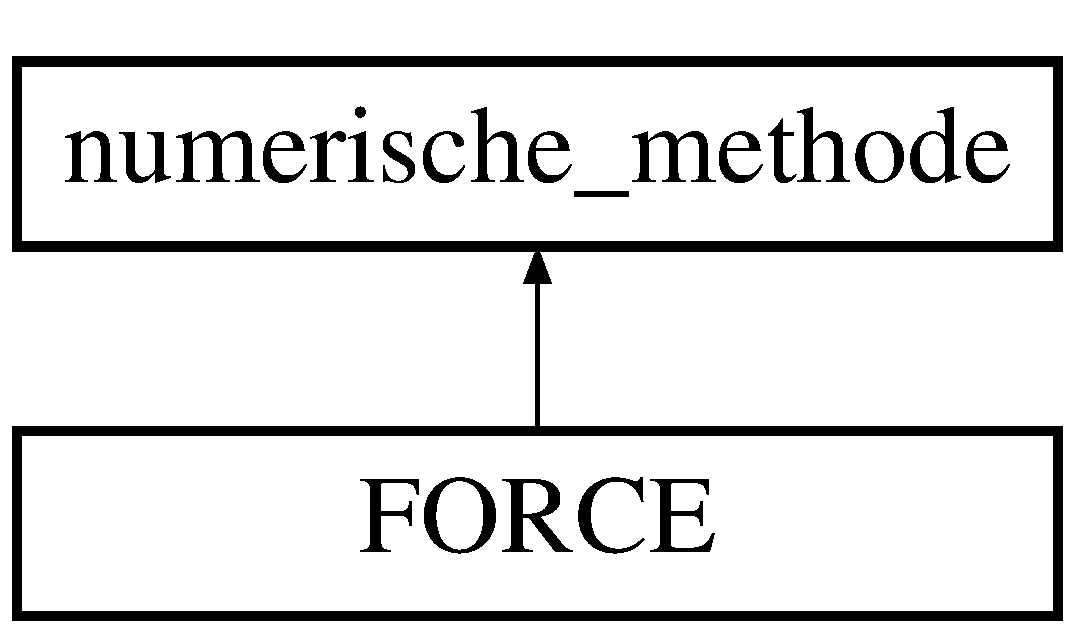
\includegraphics[height=2.000000cm]{classFORCE}
\end{center}
\end{figure}
\subsection*{Public Member Functions}
\begin{DoxyCompactItemize}
\item 
\hyperlink{classFORCE_a0dd4dcc9d89eb274f2f8ded4b3f48f89}{F\-O\-R\-C\-E} (std\-::string const\-\_\-in, std\-::string formel\-\_\-in, std\-::string save\-\_\-in)
\end{DoxyCompactItemize}
\subsection*{Protected Member Functions}
\begin{DoxyCompactItemize}
\item 
std\-::vector$<$ std\-::vector\\*
$<$ std\-::vector$<$ std\-::vector\\*
$<$ double $>$ $>$ $>$ $>$ \hyperlink{classFORCE_a03c0c50dc6e49e1d1b1f056cb76742e9}{calc\-\_\-method\-\_\-flux} (int dir)
\end{DoxyCompactItemize}
\subsection*{Additional Inherited Members}


\subsection{Detailed Description}
Klasse der \hyperlink{classFORCE}{F\-O\-R\-C\-E} Methode. 

\subsection{Constructor \& Destructor Documentation}
\hypertarget{classFORCE_a0dd4dcc9d89eb274f2f8ded4b3f48f89}{\index{F\-O\-R\-C\-E@{F\-O\-R\-C\-E}!F\-O\-R\-C\-E@{F\-O\-R\-C\-E}}
\index{F\-O\-R\-C\-E@{F\-O\-R\-C\-E}!FORCE@{F\-O\-R\-C\-E}}
\subsubsection[{F\-O\-R\-C\-E}]{\setlength{\rightskip}{0pt plus 5cm}F\-O\-R\-C\-E\-::\-F\-O\-R\-C\-E (
\begin{DoxyParamCaption}
\item[{std\-::string}]{const\-\_\-in, }
\item[{std\-::string}]{formel\-\_\-in, }
\item[{std\-::string}]{save\-\_\-in}
\end{DoxyParamCaption}
)}}\label{classFORCE_a0dd4dcc9d89eb274f2f8ded4b3f48f89}
Konstruktor der \hyperlink{classFORCE}{F\-O\-R\-C\-E} Methode. Ruft den Konstruktor der geerbten Klasse auf. 
\begin{DoxyParams}{Parameters}
{\em const\-\_\-in} & Dateiname wo \hyperlink{classKonstanten}{Konstanten} gespeichert sind. \\
\hline
{\em formel\-\_\-in} & Dateinamen-\/\-Kern für die Formeln. \\
\hline
{\em save\-\_\-in} & Dateiname wo für das Laden eine Speicherstands die Plots gespeichert sind. \\
\hline
\end{DoxyParams}


\subsection{Member Function Documentation}
\hypertarget{classFORCE_a03c0c50dc6e49e1d1b1f056cb76742e9}{\index{F\-O\-R\-C\-E@{F\-O\-R\-C\-E}!calc\-\_\-method\-\_\-flux@{calc\-\_\-method\-\_\-flux}}
\index{calc\-\_\-method\-\_\-flux@{calc\-\_\-method\-\_\-flux}!FORCE@{F\-O\-R\-C\-E}}
\subsubsection[{calc\-\_\-method\-\_\-flux}]{\setlength{\rightskip}{0pt plus 5cm}vector$<$ vector$<$ vector$<$ vector$<$ double $>$ $>$ $>$ $>$ F\-O\-R\-C\-E\-::calc\-\_\-method\-\_\-flux (
\begin{DoxyParamCaption}
\item[{int}]{dir}
\end{DoxyParamCaption}
)\hspace{0.3cm}{\ttfamily [protected]}, {\ttfamily [virtual]}}}\label{classFORCE_a03c0c50dc6e49e1d1b1f056cb76742e9}
Berechnung des \hyperlink{classFORCE}{F\-O\-R\-C\-E} Flusses. \begin{DoxyReturn}{Returns}
4 Dimensionaler Vektor. Zusammenstellung\-: Gleichung, x-\/\-Position, y-\/\-Position , dimension 
\end{DoxyReturn}


Implements \hyperlink{classnumerische__methode_af40ea9c1bfbc9d480e7e0d188f2eccf8}{numerische\-\_\-methode}.



The documentation for this class was generated from the following files\-:\begin{DoxyCompactItemize}
\item 
F\-O\-R\-C\-E.\-h\item 
F\-O\-R\-C\-E.\-cpp\end{DoxyCompactItemize}

\hypertarget{classGleichungssystem}{\section{Gleichungssystem Class Reference}
\label{classGleichungssystem}\index{Gleichungssystem@{Gleichungssystem}}
}


{\ttfamily \#include $<$Gleichungssystem.\-h$>$}

\subsection*{Public Member Functions}
\begin{DoxyCompactItemize}
\item 
\hyperlink{classGleichungssystem_ad1913547ff7dadcbe736f55fd147a022}{Gleichungssystem} (std\-::string path, \hyperlink{classKonstanten}{Konstanten} c)
\item 
void \hyperlink{classGleichungssystem_a5e5b62e0de91210b360e5d2948711f2b}{compute\-\_\-u\-\_\-1d} (double $\ast$$\ast$$\ast$\hyperlink{classGleichungssystem_a38663ae62438b07378224efaf702048c}{u}, \hyperlink{classRaster}{Raster} $\ast$raster, int $\ast$cells, int ordnung)
\item 
void \hyperlink{classGleichungssystem_a7b2cf1ff16317a8c76168187c565d4c1}{compute\-\_\-f\-\_\-1d} (double $\ast$$\ast$$\ast$f, \hyperlink{classRaster}{Raster} $\ast$raster, int $\ast$cells, int ordnung)
\item 
void \hyperlink{classGleichungssystem_a7308592c55ca251bb1131637b8fdece4}{compute\-\_\-u\-\_\-2d} (double $\ast$$\ast$$\ast$\hyperlink{classGleichungssystem_a38663ae62438b07378224efaf702048c}{u}, \hyperlink{classRaster}{Raster} $\ast$raster, int $\ast$cells, int ordnung)
\item 
void \hyperlink{classGleichungssystem_a8a96d9253908b0db7bdafb1f08e52713}{compute\-\_\-f\-\_\-2d} (double $\ast$$\ast$$\ast$f, \hyperlink{classRaster}{Raster} $\ast$raster, int $\ast$cells, int ordnung)
\item 
void \hyperlink{classGleichungssystem_a2146afb8fbed763f65dba88a77eb633a}{compute\-\_\-g\-\_\-2d} (double $\ast$$\ast$$\ast$g, \hyperlink{classRaster}{Raster} $\ast$raster, int $\ast$cells, int ordnung)
\end{DoxyCompactItemize}
\subsection*{Public Attributes}
\begin{DoxyCompactItemize}
\item 
std\-::vector$<$ std\-::string $>$ \hyperlink{classGleichungssystem_a38663ae62438b07378224efaf702048c}{u}
\item 
std\-::vector$<$ std\-::string $>$ \hyperlink{classGleichungssystem_a8b6e15e8bd9149de3cbf49c6aca116bc}{uback}
\item 
std\-::vector$<$ std\-::string $>$ \hyperlink{classGleichungssystem_aad94e01334430fe40307ed40f8e8b2e9}{f\-\_\-u}
\item 
std\-::vector$<$ std\-::string $>$ \hyperlink{classGleichungssystem_a6bd71d8aca452f5ba8dc8726e6e1bc78}{g\-\_\-u}
\item 
int \hyperlink{classGleichungssystem_adaefa4c9c8f13d106d50193d5c187677}{neqs}
\end{DoxyCompactItemize}


\subsection{Detailed Description}
Die Klasse \hyperlink{classGleichungssystem}{Gleichungssystem} verwaltet die Formelvektoren u,f\-\_\-u und s\-\_\-u. Die Formelvektoren wurden in der ursprüngliche Version als Strings in Vektoren abgespeichert, und dann mittels Funktionen der exprtk Libiary interpretiert, aber das dauerte viel zu lange 

\subsection{Constructor \& Destructor Documentation}
\hypertarget{classGleichungssystem_ad1913547ff7dadcbe736f55fd147a022}{\index{Gleichungssystem@{Gleichungssystem}!Gleichungssystem@{Gleichungssystem}}
\index{Gleichungssystem@{Gleichungssystem}!Gleichungssystem@{Gleichungssystem}}
\subsubsection[{Gleichungssystem}]{\setlength{\rightskip}{0pt plus 5cm}Gleichungssystem\-::\-Gleichungssystem (
\begin{DoxyParamCaption}
\item[{std\-::string}]{path, }
\item[{{\bf Konstanten}}]{c}
\end{DoxyParamCaption}
)}}\label{classGleichungssystem_ad1913547ff7dadcbe736f55fd147a022}
Konstruktor der klasse \hyperlink{classGleichungssystem}{Gleichungssystem}. 
\begin{DoxyParams}{Parameters}
{\em path} & Pfad zur Datei welche die Formeln enthält. \\
\hline
{\em c} & \hyperlink{classKonstanten}{Konstanten} Objekte welches für berechnungen gebraucht wird. \\
\hline
\end{DoxyParams}


\subsection{Member Function Documentation}
\hypertarget{classGleichungssystem_a7b2cf1ff16317a8c76168187c565d4c1}{\index{Gleichungssystem@{Gleichungssystem}!compute\-\_\-f\-\_\-1d@{compute\-\_\-f\-\_\-1d}}
\index{compute\-\_\-f\-\_\-1d@{compute\-\_\-f\-\_\-1d}!Gleichungssystem@{Gleichungssystem}}
\subsubsection[{compute\-\_\-f\-\_\-1d}]{\setlength{\rightskip}{0pt plus 5cm}void Gleichungssystem\-::compute\-\_\-f\-\_\-1d (
\begin{DoxyParamCaption}
\item[{double $\ast$$\ast$$\ast$}]{f, }
\item[{{\bf Raster} $\ast$}]{raster, }
\item[{int $\ast$}]{cells, }
\item[{int}]{ordnung}
\end{DoxyParamCaption}
)}}\label{classGleichungssystem_a7b2cf1ff16317a8c76168187c565d4c1}
Berechnet die Lösungen der Formel für den Fluss F in 1-\/\-D 
\begin{DoxyParams}{Parameters}
{\em f,3-\/d} & Feld für die F-\/\-Werte \\
\hline
{\em \hyperlink{classRaster}{Raster},welche} & die Werte zur Berechnung enthält. \\
\hline
{\em cells,Ausdehnung} & des Gitters \\
\hline
{\em ordnung} & des Algorithmus, wichtig für die Ausdehnung des Gitters \\
\hline
\end{DoxyParams}
\hypertarget{classGleichungssystem_a8a96d9253908b0db7bdafb1f08e52713}{\index{Gleichungssystem@{Gleichungssystem}!compute\-\_\-f\-\_\-2d@{compute\-\_\-f\-\_\-2d}}
\index{compute\-\_\-f\-\_\-2d@{compute\-\_\-f\-\_\-2d}!Gleichungssystem@{Gleichungssystem}}
\subsubsection[{compute\-\_\-f\-\_\-2d}]{\setlength{\rightskip}{0pt plus 5cm}void Gleichungssystem\-::compute\-\_\-f\-\_\-2d (
\begin{DoxyParamCaption}
\item[{double $\ast$$\ast$$\ast$}]{f, }
\item[{{\bf Raster} $\ast$}]{raster, }
\item[{int $\ast$}]{cells, }
\item[{int}]{ordnung}
\end{DoxyParamCaption}
)}}\label{classGleichungssystem_a8a96d9253908b0db7bdafb1f08e52713}
Berechnet die Lösungen der Formel für den Fluss F in 2-\/\-D 
\begin{DoxyParams}{Parameters}
{\em f,3-\/d} & Feld für die F-\/\-Werte \\
\hline
{\em \hyperlink{classRaster}{Raster},welche} & die Werte zur Berechnung enthält. \\
\hline
{\em cells,Ausdehnung} & des Gitters \\
\hline
{\em ordnung} & des Algorithmus, wichtig für die Ausdehnung des Gitters \\
\hline
\end{DoxyParams}
\hypertarget{classGleichungssystem_a2146afb8fbed763f65dba88a77eb633a}{\index{Gleichungssystem@{Gleichungssystem}!compute\-\_\-g\-\_\-2d@{compute\-\_\-g\-\_\-2d}}
\index{compute\-\_\-g\-\_\-2d@{compute\-\_\-g\-\_\-2d}!Gleichungssystem@{Gleichungssystem}}
\subsubsection[{compute\-\_\-g\-\_\-2d}]{\setlength{\rightskip}{0pt plus 5cm}void Gleichungssystem\-::compute\-\_\-g\-\_\-2d (
\begin{DoxyParamCaption}
\item[{double $\ast$$\ast$$\ast$}]{g, }
\item[{{\bf Raster} $\ast$}]{raster, }
\item[{int $\ast$}]{cells, }
\item[{int}]{ordnung}
\end{DoxyParamCaption}
)}}\label{classGleichungssystem_a2146afb8fbed763f65dba88a77eb633a}
Berechnet die Lösungen der Formel für den Fluss G in 2-\/\-D 
\begin{DoxyParams}{Parameters}
{\em \hyperlink{classRaster}{Raster},welche} & die Werte zur Berechnung enthält. \\
\hline
{\em cells,Ausdehnung} & des Gitters \\
\hline
{\em ordnung} & des Algorithmus, wichtig für die Ausdehnung des Gitters\\
\hline
\end{DoxyParams}
Berechnet die Lösungen der Formel für den Fluss G in 2-\/\-D 
\begin{DoxyParams}{Parameters}
{\em g,3-\/d} & Feld für die G-\/\-Werte \\
\hline
{\em \hyperlink{classRaster}{Raster},welche} & die Werte zur Berechnung enthält. \\
\hline
{\em cells,Ausdehnung} & des Gitters \\
\hline
{\em ordnung} & des Algorithmus, wichtig für die Ausdehnung des Gitters \\
\hline
\end{DoxyParams}
\hypertarget{classGleichungssystem_a5e5b62e0de91210b360e5d2948711f2b}{\index{Gleichungssystem@{Gleichungssystem}!compute\-\_\-u\-\_\-1d@{compute\-\_\-u\-\_\-1d}}
\index{compute\-\_\-u\-\_\-1d@{compute\-\_\-u\-\_\-1d}!Gleichungssystem@{Gleichungssystem}}
\subsubsection[{compute\-\_\-u\-\_\-1d}]{\setlength{\rightskip}{0pt plus 5cm}void Gleichungssystem\-::compute\-\_\-u\-\_\-1d (
\begin{DoxyParamCaption}
\item[{double $\ast$$\ast$$\ast$}]{u, }
\item[{{\bf Raster} $\ast$}]{raster, }
\item[{int $\ast$}]{cells, }
\item[{int}]{ordnung}
\end{DoxyParamCaption}
)}}\label{classGleichungssystem_a5e5b62e0de91210b360e5d2948711f2b}
Berechnet die Werte U in 1-\/\-D 
\begin{DoxyParams}{Parameters}
{\em u,3-\/d} & Feld für die U-\/\-Werte \\
\hline
{\em \hyperlink{classRaster}{Raster},welche} & die Werte zur Berechnung enthält. \\
\hline
{\em cells,Ausdehnung} & des Gitters \\
\hline
{\em ordnung} & des Algorithmus, wichtig für die Ausdehnung des Gitters\\
\hline
\end{DoxyParams}
Berechnet die Werte U in 1-\/\-D 
\begin{DoxyParams}{Parameters}
{\em u,3-\/d} & Feld für die U-\/\-Werte \\
\hline
{\em raster,welche} & die Werte zur Berechnung enthält. \\
\hline
{\em cells,Ausdehnung} & des Gitters \\
\hline
{\em ordnung} & des Algorithmus, wichtig für die Ausdehnung des Gitters \\
\hline
\end{DoxyParams}
\hypertarget{classGleichungssystem_a7308592c55ca251bb1131637b8fdece4}{\index{Gleichungssystem@{Gleichungssystem}!compute\-\_\-u\-\_\-2d@{compute\-\_\-u\-\_\-2d}}
\index{compute\-\_\-u\-\_\-2d@{compute\-\_\-u\-\_\-2d}!Gleichungssystem@{Gleichungssystem}}
\subsubsection[{compute\-\_\-u\-\_\-2d}]{\setlength{\rightskip}{0pt plus 5cm}void Gleichungssystem\-::compute\-\_\-u\-\_\-2d (
\begin{DoxyParamCaption}
\item[{double $\ast$$\ast$$\ast$}]{u, }
\item[{{\bf Raster} $\ast$}]{raster, }
\item[{int $\ast$}]{cells, }
\item[{int}]{ordnung}
\end{DoxyParamCaption}
)}}\label{classGleichungssystem_a7308592c55ca251bb1131637b8fdece4}
Berechnet die Werte U in 2-\/\-D 
\begin{DoxyParams}{Parameters}
{\em u,3-\/d} & Feld für die U-\/\-Werte \\
\hline
{\em \hyperlink{classRaster}{Raster},welche} & die Werte zur Berechnung enthält. \\
\hline
{\em cells,Ausdehnung} & des Gitters \\
\hline
{\em ordnung} & des Algorithmus, wichtig für die Ausdehnung des Gitters \\
\hline
\end{DoxyParams}


\subsection{Member Data Documentation}
\hypertarget{classGleichungssystem_aad94e01334430fe40307ed40f8e8b2e9}{\index{Gleichungssystem@{Gleichungssystem}!f\-\_\-u@{f\-\_\-u}}
\index{f\-\_\-u@{f\-\_\-u}!Gleichungssystem@{Gleichungssystem}}
\subsubsection[{f\-\_\-u}]{\setlength{\rightskip}{0pt plus 5cm}std\-::vector$<$std\-::string$>$ Gleichungssystem\-::f\-\_\-u}}\label{classGleichungssystem_aad94e01334430fe40307ed40f8e8b2e9}
Vektor der Formeln von f\-\_\-u. \hypertarget{classGleichungssystem_a6bd71d8aca452f5ba8dc8726e6e1bc78}{\index{Gleichungssystem@{Gleichungssystem}!g\-\_\-u@{g\-\_\-u}}
\index{g\-\_\-u@{g\-\_\-u}!Gleichungssystem@{Gleichungssystem}}
\subsubsection[{g\-\_\-u}]{\setlength{\rightskip}{0pt plus 5cm}std\-::vector$<$std\-::string$>$ Gleichungssystem\-::g\-\_\-u}}\label{classGleichungssystem_a6bd71d8aca452f5ba8dc8726e6e1bc78}
Vektor der Formeln von g\-\_\-u. \hypertarget{classGleichungssystem_adaefa4c9c8f13d106d50193d5c187677}{\index{Gleichungssystem@{Gleichungssystem}!neqs@{neqs}}
\index{neqs@{neqs}!Gleichungssystem@{Gleichungssystem}}
\subsubsection[{neqs}]{\setlength{\rightskip}{0pt plus 5cm}int Gleichungssystem\-::neqs}}\label{classGleichungssystem_adaefa4c9c8f13d106d50193d5c187677}
Anzahl der Gleichungen \hypertarget{classGleichungssystem_a38663ae62438b07378224efaf702048c}{\index{Gleichungssystem@{Gleichungssystem}!u@{u}}
\index{u@{u}!Gleichungssystem@{Gleichungssystem}}
\subsubsection[{u}]{\setlength{\rightskip}{0pt plus 5cm}std\-::vector$<$std\-::string$>$ Gleichungssystem\-::u}}\label{classGleichungssystem_a38663ae62438b07378224efaf702048c}
Vektor von u \hypertarget{classGleichungssystem_a8b6e15e8bd9149de3cbf49c6aca116bc}{\index{Gleichungssystem@{Gleichungssystem}!uback@{uback}}
\index{uback@{uback}!Gleichungssystem@{Gleichungssystem}}
\subsubsection[{uback}]{\setlength{\rightskip}{0pt plus 5cm}std\-::vector$<$std\-::string$>$ Gleichungssystem\-::uback}}\label{classGleichungssystem_a8b6e15e8bd9149de3cbf49c6aca116bc}
Rückrechnung der erhaltenen Variablen in die physikalischen. 

The documentation for this class was generated from the following files\-:\begin{DoxyCompactItemize}
\item 
Gleichungssystem.\-h\item 
Gleichungssystem.\-cpp\end{DoxyCompactItemize}

\hypertarget{classKonstanten}{\section{Konstanten Class Reference}
\label{classKonstanten}\index{Konstanten@{Konstanten}}
}


{\ttfamily \#include $<$Konstanten.\-h$>$}

\subsection*{Public Member Functions}
\begin{DoxyCompactItemize}
\item 
\hyperlink{classKonstanten_a4a5a2fac8680b4cf055029be43f4c18c}{Konstanten} (std\-::string input\-\_\-const)
\end{DoxyCompactItemize}
\subsection*{Public Attributes}
\begin{DoxyCompactItemize}
\item 
std\-::vector$<$ std\-::string $>$ \hyperlink{classKonstanten_abd044489471f59656078d51706353bf5}{const\-\_\-name}
\item 
std\-::vector$<$ double $>$ \hyperlink{classKonstanten_a12dc216c8d055e95ed17d819a5949832}{const\-\_\-value}
\item 
\hypertarget{classKonstanten_a79a04aec0180007251b811999e5107b8}{int {\bfseries calceigv}}\label{classKonstanten_a79a04aec0180007251b811999e5107b8}

\item 
\hypertarget{classKonstanten_a2cfd196ff2e81d46929c3efdd00ec62c}{int {\bfseries variante}}\label{classKonstanten_a2cfd196ff2e81d46929c3efdd00ec62c}

\item 
\hypertarget{classKonstanten_a987274e0e5793520b7a445ed9873c3bf}{double {\bfseries teiler}}\label{classKonstanten_a987274e0e5793520b7a445ed9873c3bf}

\item 
\hypertarget{classKonstanten_ae3edf7d78df231706cf8e76244391cab}{int {\bfseries teilerend}}\label{classKonstanten_ae3edf7d78df231706cf8e76244391cab}

\item 
\hypertarget{classKonstanten_a84dfdf3a59e6c5affa98be399569b01a}{double {\bfseries timeou}}\label{classKonstanten_a84dfdf3a59e6c5affa98be399569b01a}

\item 
\hypertarget{classKonstanten_a028517c1cbc7e062a31fb7d204f64a96}{double {\bfseries cfl}}\label{classKonstanten_a028517c1cbc7e062a31fb7d204f64a96}

\item 
\hypertarget{classKonstanten_af02b3d81b23fb756a7821550f17f5817}{int {\bfseries maxnt}}\label{classKonstanten_af02b3d81b23fb756a7821550f17f5817}

\item 
\hypertarget{classKonstanten_ad24e5c861894ff6df3368fbe28ecee56}{int {\bfseries dimension}}\label{classKonstanten_ad24e5c861894ff6df3368fbe28ecee56}

\item 
\hypertarget{classKonstanten_a2d407c35f20f0bf27c2152ed67cb0851}{int {\bfseries ordnung}}\label{classKonstanten_a2d407c35f20f0bf27c2152ed67cb0851}

\item 
\hypertarget{classKonstanten_a3f97bdddf7c7bad19afb456167496471}{double {\bfseries radius}}\label{classKonstanten_a3f97bdddf7c7bad19afb456167496471}

\item 
\hypertarget{classKonstanten_af28f753eda4f33bee6be6844519641ed}{int {\bfseries C\-E\-L\-L\-S\-X}}\label{classKonstanten_af28f753eda4f33bee6be6844519641ed}

\item 
\hypertarget{classKonstanten_aa68cbb100282389bd7fc9efdc5cf04da}{int {\bfseries C\-E\-L\-L\-S\-Y}}\label{classKonstanten_aa68cbb100282389bd7fc9efdc5cf04da}

\item 
\hypertarget{classKonstanten_a8e03c316cd153326b83120e7f69ac9cc}{double {\bfseries g}}\label{classKonstanten_a8e03c316cd153326b83120e7f69ac9cc}

\item 
\hypertarget{classKonstanten_a7a48e3cf7787f8a77f6fa0d073967229}{double {\bfseries mol}}\label{classKonstanten_a7a48e3cf7787f8a77f6fa0d073967229}

\item 
\hypertarget{classKonstanten_ad0f8a36eab29909dbe37d1baf9db3542}{double {\bfseries mor}}\label{classKonstanten_ad0f8a36eab29909dbe37d1baf9db3542}

\item 
\hypertarget{classKonstanten_af1912a9942b66bc8e2965840f0dcef08}{double {\bfseries mul}}\label{classKonstanten_af1912a9942b66bc8e2965840f0dcef08}

\item 
\hypertarget{classKonstanten_a062ce50d35bd692ab4b492cf40225ff3}{double {\bfseries mur}}\label{classKonstanten_a062ce50d35bd692ab4b492cf40225ff3}

\item 
\hypertarget{classKonstanten_a7a85280fdf83d10bf3a14f3f772bef2a}{int {\bfseries upbc}}\label{classKonstanten_a7a85280fdf83d10bf3a14f3f772bef2a}

\item 
\hypertarget{classKonstanten_a55f2f34f199cf5c377280272350695c4}{int {\bfseries downbc}}\label{classKonstanten_a55f2f34f199cf5c377280272350695c4}

\item 
\hypertarget{classKonstanten_a1906cb7c990779e92707cc752358e7ca}{int {\bfseries leftbc}}\label{classKonstanten_a1906cb7c990779e92707cc752358e7ca}

\item 
\hypertarget{classKonstanten_aedc6f7a6f365ad1c42b0bb58c14d0d5f}{int {\bfseries rightbc}}\label{classKonstanten_aedc6f7a6f365ad1c42b0bb58c14d0d5f}

\item 
\hypertarget{classKonstanten_a8a8ba974eadebfd1baa2d7246d1eadf8}{double {\bfseries cref}}\label{classKonstanten_a8a8ba974eadebfd1baa2d7246d1eadf8}

\item 
\hypertarget{classKonstanten_a45f2dc4cdb262f34f256f0418b2d9b20}{double {\bfseries done}}\label{classKonstanten_a45f2dc4cdb262f34f256f0418b2d9b20}

\item 
\hypertarget{classKonstanten_a4fd1dc55cc0b72a05426aae1cf0b3902}{double {\bfseries ccl}}\label{classKonstanten_a4fd1dc55cc0b72a05426aae1cf0b3902}

\item 
\hypertarget{classKonstanten_aba36196bc1a291ad9176f73c0b607677}{double {\bfseries rhol}}\label{classKonstanten_aba36196bc1a291ad9176f73c0b607677}

\item 
\hypertarget{classKonstanten_aec1cce17aadacf240ace975f68727f21}{double {\bfseries vl}}\label{classKonstanten_aec1cce17aadacf240ace975f68727f21}

\item 
\hypertarget{classKonstanten_a44b6880e75797d69346c5c8212124952}{double {\bfseries vrl}}\label{classKonstanten_a44b6880e75797d69346c5c8212124952}

\item 
\hypertarget{classKonstanten_a8a9d76a1177266158c2fa3900484d244}{double {\bfseries vyl}}\label{classKonstanten_a8a9d76a1177266158c2fa3900484d244}

\item 
\hypertarget{classKonstanten_ac4bd60cb7712a4230c70a8d1d481c8ec}{double {\bfseries vyrl}}\label{classKonstanten_ac4bd60cb7712a4230c70a8d1d481c8ec}

\item 
\hypertarget{classKonstanten_ae1a2831635cbd559716dca269849823b}{double {\bfseries rhor}}\label{classKonstanten_ae1a2831635cbd559716dca269849823b}

\item 
\hypertarget{classKonstanten_a45cb5090ba21586b7db67424f2ac9e97}{double {\bfseries vr}}\label{classKonstanten_a45cb5090ba21586b7db67424f2ac9e97}

\item 
\hypertarget{classKonstanten_afc3cd7105f50e81e25277cdd902b2410}{double {\bfseries vrr}}\label{classKonstanten_afc3cd7105f50e81e25277cdd902b2410}

\item 
\hypertarget{classKonstanten_a326d4d4c71f750ef4a0173669634b770}{double {\bfseries vyr}}\label{classKonstanten_a326d4d4c71f750ef4a0173669634b770}

\item 
\hypertarget{classKonstanten_a83f4e7a4cfc3087cb683d556d178951a}{double {\bfseries vyrr}}\label{classKonstanten_a83f4e7a4cfc3087cb683d556d178951a}

\end{DoxyCompactItemize}


\subsection{Detailed Description}
Die Klasse \hyperlink{classKonstanten}{Konstanten} dient hauptsächlich dazu sämtliche für Berechnungen benötigte \hyperlink{classKonstanten}{Konstanten} zusammenzufassen und leicht für Rechnungen verfügbar zu machen. 

\subsection{Constructor \& Destructor Documentation}
\hypertarget{classKonstanten_a4a5a2fac8680b4cf055029be43f4c18c}{\index{Konstanten@{Konstanten}!Konstanten@{Konstanten}}
\index{Konstanten@{Konstanten}!Konstanten@{Konstanten}}
\subsubsection[{Konstanten}]{\setlength{\rightskip}{0pt plus 5cm}Konstanten\-::\-Konstanten (
\begin{DoxyParamCaption}
\item[{std\-::string}]{input\-\_\-const}
\end{DoxyParamCaption}
)}}\label{classKonstanten_a4a5a2fac8680b4cf055029be43f4c18c}
Konstruktor. Setzt die \hyperlink{classKonstanten}{Konstanten}. 
\begin{DoxyParams}{Parameters}
{\em input\-\_\-const} & String des Pfades zu den festen \hyperlink{classKonstanten}{Konstanten}. \\
\hline
{\em input\-\_\-calc} & String des Pfades zu den einmalig zu berechnenden \hyperlink{classKonstanten}{Konstanten}.\\
\hline
\end{DoxyParams}
Konstruktor. 
\begin{DoxyParams}{Parameters}
{\em input\-\_\-const} & String des Pfades zu den festen \hyperlink{classKonstanten}{Konstanten}. \\
\hline
{\em input\-\_\-calc} & String des Pfades zu den einmalig zu berechnenden \hyperlink{classKonstanten}{Konstanten}. \\
\hline
\end{DoxyParams}


\subsection{Member Data Documentation}
\hypertarget{classKonstanten_abd044489471f59656078d51706353bf5}{\index{Konstanten@{Konstanten}!const\-\_\-name@{const\-\_\-name}}
\index{const\-\_\-name@{const\-\_\-name}!Konstanten@{Konstanten}}
\subsubsection[{const\-\_\-name}]{\setlength{\rightskip}{0pt plus 5cm}std\-::vector$<$std\-::string$>$ Konstanten\-::const\-\_\-name}}\label{classKonstanten_abd044489471f59656078d51706353bf5}
Beizeichnungen der \hyperlink{classKonstanten}{Konstanten} in einem Vektor. \hypertarget{classKonstanten_a12dc216c8d055e95ed17d819a5949832}{\index{Konstanten@{Konstanten}!const\-\_\-value@{const\-\_\-value}}
\index{const\-\_\-value@{const\-\_\-value}!Konstanten@{Konstanten}}
\subsubsection[{const\-\_\-value}]{\setlength{\rightskip}{0pt plus 5cm}std\-::vector$<$double$>$ Konstanten\-::const\-\_\-value}}\label{classKonstanten_a12dc216c8d055e95ed17d819a5949832}
Vektor von Werten der \hyperlink{classKonstanten}{Konstanten}. 

The documentation for this class was generated from the following files\-:\begin{DoxyCompactItemize}
\item 
Konstanten.\-h\item 
Konstanten.\-cpp\end{DoxyCompactItemize}

\hypertarget{classLaxFriedrichMethod}{\section{Lax\-Friedrich\-Method Class Reference}
\label{classLaxFriedrichMethod}\index{Lax\-Friedrich\-Method@{Lax\-Friedrich\-Method}}
}


{\ttfamily \#include $<$lax\-\_\-friedrich.\-h$>$}



\subsection{Detailed Description}
Klasse der Lax-\/\-Friedrichs Methode. Die Berechnung des Lax-\/\-Friedrich Flusses wird hier spezialisiert, rest wird von der Klasse numerische\-\_\-methode geerbt. 

The documentation for this class was generated from the following file\-:\begin{DoxyCompactItemize}
\item 
lax\-\_\-friedrich.\-h\end{DoxyCompactItemize}

\hypertarget{classnumerische__methode}{\section{numerische\-\_\-methode Class Reference}
\label{classnumerische__methode}\index{numerische\-\_\-methode@{numerische\-\_\-methode}}
}


{\ttfamily \#include $<$numerische\-\_\-methode.\-h$>$}

Inheritance diagram for numerische\-\_\-methode\-:\begin{figure}[H]
\begin{center}
\leavevmode
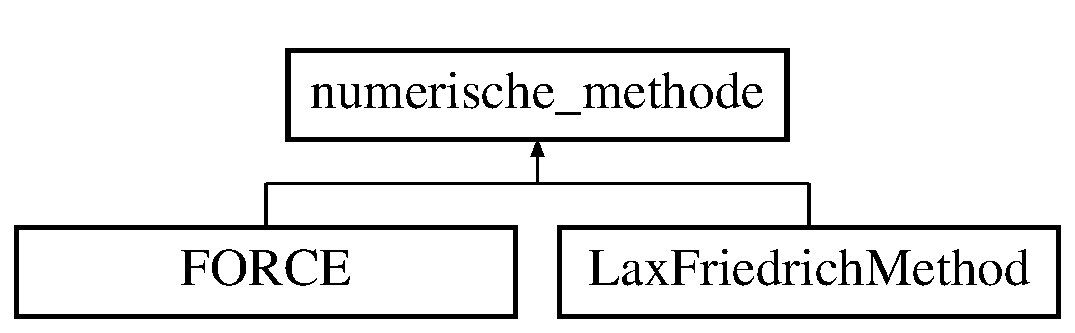
\includegraphics[height=2.000000cm]{classnumerische__methode}
\end{center}
\end{figure}
\subsection*{Public Member Functions}
\begin{DoxyCompactItemize}
\item 
\hyperlink{classnumerische__methode_ae3d1f1d622e07a1ef02aeb6e3ee07811}{numerische\-\_\-methode} (std\-::string method, std\-::string const\-\_\-in, std\-::string formel\-\_\-in, std\-::string save\-\_\-in)
\item 
void \hyperlink{classnumerische__methode_a83d6b8c73e8afc831003b8abc334e185}{start\-\_\-method} ()
\end{DoxyCompactItemize}
\subsection*{Protected Member Functions}
\begin{DoxyCompactItemize}
\item 
double \hyperlink{classnumerische__methode_ab6fbf44af8c83d66710ec2f500c121aa}{cflcon} (int n, double time)
\item 
virtual std\-::vector\\*
$<$ std\-::vector$<$ std\-::vector\\*
$<$ std\-::vector$<$ double $>$ $>$ $>$ $>$ \hyperlink{classnumerische__methode_af40ea9c1bfbc9d480e7e0d188f2eccf8}{calc\-\_\-method\-\_\-flux} (int dir)=0
\item 
void \hyperlink{classnumerische__methode_a46867c6648593607c3c596a3eb34402b}{update} (std\-::vector$<$ std\-::vector$<$ std\-::vector$<$ std\-::vector$<$ double $>$ $>$ $>$ $>$fi, int dir)
\item 
void \hyperlink{classnumerische__methode_a25747305213c9a3a54fbc2f1ca5c0113}{write} ()
\item 
void \hyperlink{classnumerische__methode_a0730ea8b5f2561d5bd2474ea0a34a531}{matrix\-\_\-1d} (double $\ast$values, int n, double uone, double utwo, double uthree, double p, double done, double dtwo, double ccl, double \hyperlink{classnumerische__methode_a8adb2a525c7877c531fa960ee5f0176b}{g}, double \hyperlink{classnumerische__methode_aec540b2a47bbc7318f511583087c5498}{ct}, double cref, int \hyperlink{classnumerische__methode_a98b4b3256bbcd2306acbe4d69f5258f7}{variante})
\item 
void \hyperlink{classnumerische__methode_a1ed1a084c11e18bb8fc3beadc2a793e7}{matrix\-\_\-2d} (double $\ast$values\-\_\-x, double $\ast$values\-\_\-y, int n, double uone, double utwo, double uthree, double ufour, double ufive, double p, double done, double dtwo, double ccl, double \hyperlink{classnumerische__methode_a8adb2a525c7877c531fa960ee5f0176b}{g}, double \hyperlink{classnumerische__methode_aec540b2a47bbc7318f511583087c5498}{ct}, double cref)
\end{DoxyCompactItemize}
\subsection*{Protected Attributes}
\begin{DoxyCompactItemize}
\item 
std\-::string \hyperlink{classnumerische__methode_a08429f7cae828958ced4b62db2cf1021}{name}
\item 
int $\ast$ \hyperlink{classnumerische__methode_a896a9488a1b7593e4312fa102264c280}{C\-E\-L\-L\-S}
\item 
double \hyperlink{classnumerische__methode_a8adb2a525c7877c531fa960ee5f0176b}{g}
\item 
double \hyperlink{classnumerische__methode_af0e0a81815451c4ed37f0ad73d4c5dbe}{timeou}
\item 
double \hyperlink{classnumerische__methode_aec540b2a47bbc7318f511583087c5498}{ct}
\item 
int \hyperlink{classnumerische__methode_a5a52e194b395d083422d9b03e72d3d5f}{dimension}
\item 
int \hyperlink{classnumerische__methode_a70e5afff7bb50109856ce5bf2e62f072}{splitting}
\item 
int \hyperlink{classnumerische__methode_ab95e5de8e6d9d0a63e4110dea60825e8}{ordnung}
\item 
int \hyperlink{classnumerische__methode_a4c5bac9002b5bc6ab4c5eac30943246a}{steps}
\item 
int \hyperlink{classnumerische__methode_ae52e51b4b4607ee26d4cc9bac2f61922}{maxnt}
\item 
double \hyperlink{classnumerische__methode_a073f2f281300eebad11d25e6a2e4a481}{dt}
\item 
double \hyperlink{classnumerische__methode_a4f188b1788413cb68a14dbe1d8a5846a}{dt\-\_\-fixed}
\item 
double \hyperlink{classnumerische__methode_af35cb44a6bdcfed96bdcee642aa7f67e}{dx}
\item 
double \hyperlink{classnumerische__methode_ae3738842c0b0203293161f8389454227}{teiler}
\item 
double \hyperlink{classnumerische__methode_af29a77417f125560c1797aed70cd7ad5}{teilerend}
\item 
double \hyperlink{classnumerische__methode_a6668ec54293e469ff9c169dfbb72e3d4}{dy}
\item 
int \hyperlink{classnumerische__methode_a6ffb8741f1f1d5975994cb006d436d8f}{mol}
\item 
int \hyperlink{classnumerische__methode_ab33e0205421976197d24355cf010bfe8}{mor}
\item 
int \hyperlink{classnumerische__methode_a20e0d47e90b9a0f9a83aab2b225a4616}{mul}
\item 
int \hyperlink{classnumerische__methode_a36f2c35ed9b3448c6bb8656e057ae44a}{mur}
\item 
int \hyperlink{classnumerische__methode_a98b4b3256bbcd2306acbe4d69f5258f7}{variante}
\item 
\hyperlink{classKonstanten}{Konstanten} \hyperlink{classnumerische__methode_a54c65c639dc4ea722d6f84ed6ff4c75b}{konstanten}
\item 
\hyperlink{classRaster}{Raster} \hyperlink{classnumerische__methode_ad68a4b94b3246043db399adf04959ab6}{raster}
\item 
\hyperlink{classGleichungssystem}{Gleichungssystem} \hyperlink{classnumerische__methode_ae9920302fb4e0fae9f055c0dcdff8b5a}{gs}
\end{DoxyCompactItemize}


\subsection{Detailed Description}
Die abstrakte Klasse \hyperlink{classnumerische__methode}{numerische\-\_\-methode} gibt den Rahmen für alle erbenden numerischen Methoden vor. 

\subsection{Constructor \& Destructor Documentation}
\hypertarget{classnumerische__methode_ae3d1f1d622e07a1ef02aeb6e3ee07811}{\index{numerische\-\_\-methode@{numerische\-\_\-methode}!numerische\-\_\-methode@{numerische\-\_\-methode}}
\index{numerische\-\_\-methode@{numerische\-\_\-methode}!numerische_methode@{numerische\-\_\-methode}}
\subsubsection[{numerische\-\_\-methode}]{\setlength{\rightskip}{0pt plus 5cm}numerische\-\_\-methode\-::numerische\-\_\-methode (
\begin{DoxyParamCaption}
\item[{std\-::string}]{method, }
\item[{std\-::string}]{const\-\_\-in, }
\item[{std\-::string}]{formel\-\_\-in, }
\item[{std\-::string}]{save\-\_\-in}
\end{DoxyParamCaption}
)}}\label{classnumerische__methode_ae3d1f1d622e07a1ef02aeb6e3ee07811}
Konstruktor. 
\begin{DoxyParams}{Parameters}
{\em dim} & Setzt Dimension für die Berechnung. \\
\hline
{\em ordn} & Ordnung der numerischen Methode. \\
\hline
{\em cells} & Anzahl der Zellen. \\
\hline
{\em method} & Name der Methode für unterscheidung bei Output.\\
\hline
\end{DoxyParams}
Konstruktor. 
\begin{DoxyParams}{Parameters}
{\em dim} & Setzt Dimension für die Berechnung. \\
\hline
{\em ordn} & Ordnung der numerischen Methode. \\
\hline
{\em cells} & Anzahl der Zellen. \\
\hline
{\em method} & Name der Methode für unterscheidung bei Output. 1 \\
\hline
\end{DoxyParams}


\subsection{Member Function Documentation}
\hypertarget{classnumerische__methode_af40ea9c1bfbc9d480e7e0d188f2eccf8}{\index{numerische\-\_\-methode@{numerische\-\_\-methode}!calc\-\_\-method\-\_\-flux@{calc\-\_\-method\-\_\-flux}}
\index{calc\-\_\-method\-\_\-flux@{calc\-\_\-method\-\_\-flux}!numerische_methode@{numerische\-\_\-methode}}
\subsubsection[{calc\-\_\-method\-\_\-flux}]{\setlength{\rightskip}{0pt plus 5cm}virtual std\-::vector$<$ std\-::vector$<$ std\-::vector$<$ std\-::vector $<$double$>$ $>$ $>$ $>$ numerische\-\_\-methode\-::calc\-\_\-method\-\_\-flux (
\begin{DoxyParamCaption}
\item[{int}]{dir}
\end{DoxyParamCaption}
)\hspace{0.3cm}{\ttfamily [protected]}, {\ttfamily [pure virtual]}}}\label{classnumerische__methode_af40ea9c1bfbc9d480e7e0d188f2eccf8}
Abstrakte methode zur berechnung des Flusses der jeweiligen numerischen Methode. \begin{DoxyReturn}{Returns}
Matrix der Flüsse (1\-D) 
\end{DoxyReturn}


Implemented in \hyperlink{classFORCE_a03c0c50dc6e49e1d1b1f056cb76742e9}{F\-O\-R\-C\-E}, and \hyperlink{classLaxFriedrichMethod_adce098f2eeca3bc185f0f316113abd4b}{Lax\-Friedrich\-Method}.

\hypertarget{classnumerische__methode_ab6fbf44af8c83d66710ec2f500c121aa}{\index{numerische\-\_\-methode@{numerische\-\_\-methode}!cflcon@{cflcon}}
\index{cflcon@{cflcon}!numerische_methode@{numerische\-\_\-methode}}
\subsubsection[{cflcon}]{\setlength{\rightskip}{0pt plus 5cm}double numerische\-\_\-methode\-::cflcon (
\begin{DoxyParamCaption}
\item[{int}]{n, }
\item[{double}]{time}
\end{DoxyParamCaption}
)\hspace{0.3cm}{\ttfamily [protected]}}}\label{classnumerische__methode_ab6fbf44af8c83d66710ec2f500c121aa}
C\-F\-L Bedingung anwenden und neue Zeit berechnen. 
\begin{DoxyParams}{Parameters}
{\em n} & aktueller Zeitschritt. \\
\hline
{\em time} & aktuelle Zeit. \\
\hline
\end{DoxyParams}
\begin{DoxyReturn}{Returns}
neue Zeit. 
\end{DoxyReturn}
\hypertarget{classnumerische__methode_a0730ea8b5f2561d5bd2474ea0a34a531}{\index{numerische\-\_\-methode@{numerische\-\_\-methode}!matrix\-\_\-1d@{matrix\-\_\-1d}}
\index{matrix\-\_\-1d@{matrix\-\_\-1d}!numerische_methode@{numerische\-\_\-methode}}
\subsubsection[{matrix\-\_\-1d}]{\setlength{\rightskip}{0pt plus 5cm}void numerische\-\_\-methode\-::matrix\-\_\-1d (
\begin{DoxyParamCaption}
\item[{double $\ast$}]{values, }
\item[{int}]{n, }
\item[{double}]{uone, }
\item[{double}]{utwo, }
\item[{double}]{uthree, }
\item[{double}]{p, }
\item[{double}]{done, }
\item[{double}]{dtwo, }
\item[{double}]{ccl, }
\item[{double}]{g, }
\item[{double}]{ct, }
\item[{double}]{cref, }
\item[{int}]{variante}
\end{DoxyParamCaption}
)\hspace{0.3cm}{\ttfamily [protected]}}}\label{classnumerische__methode_a0730ea8b5f2561d5bd2474ea0a34a531}
bestimmt die Elemente der Jacobi-\/\-Matrix in 3 Varianten, abhängig von der Wahl der E\-O\-S

Jacobi-\/\-Matrix für den 1-\/d Fall \hypertarget{classnumerische__methode_a1ed1a084c11e18bb8fc3beadc2a793e7}{\index{numerische\-\_\-methode@{numerische\-\_\-methode}!matrix\-\_\-2d@{matrix\-\_\-2d}}
\index{matrix\-\_\-2d@{matrix\-\_\-2d}!numerische_methode@{numerische\-\_\-methode}}
\subsubsection[{matrix\-\_\-2d}]{\setlength{\rightskip}{0pt plus 5cm}void numerische\-\_\-methode\-::matrix\-\_\-2d (
\begin{DoxyParamCaption}
\item[{double $\ast$}]{values\-\_\-x, }
\item[{double $\ast$}]{values\-\_\-y, }
\item[{int}]{n, }
\item[{double}]{uone, }
\item[{double}]{utwo, }
\item[{double}]{uthree, }
\item[{double}]{ufour, }
\item[{double}]{ufive, }
\item[{double}]{p, }
\item[{double}]{done, }
\item[{double}]{dtwo, }
\item[{double}]{ccl, }
\item[{double}]{g, }
\item[{double}]{ct, }
\item[{double}]{cref}
\end{DoxyParamCaption}
)\hspace{0.3cm}{\ttfamily [protected]}}}\label{classnumerische__methode_a1ed1a084c11e18bb8fc3beadc2a793e7}
bestimmt die Elemente der Jacobi-\/\-Matrix in 3 Varianten, abhängig von der Wahl der E\-O\-S

Jacobi-\/\-Matrix für den 2-\/d Fall in x-\/ und y-\/\-Richtung \hypertarget{classnumerische__methode_a83d6b8c73e8afc831003b8abc334e185}{\index{numerische\-\_\-methode@{numerische\-\_\-methode}!start\-\_\-method@{start\-\_\-method}}
\index{start\-\_\-method@{start\-\_\-method}!numerische_methode@{numerische\-\_\-methode}}
\subsubsection[{start\-\_\-method}]{\setlength{\rightskip}{0pt plus 5cm}void numerische\-\_\-methode\-::start\-\_\-method (
\begin{DoxyParamCaption}
{}
\end{DoxyParamCaption}
)}}\label{classnumerische__methode_a83d6b8c73e8afc831003b8abc334e185}
Startet die Berechnung. \hypertarget{classnumerische__methode_a46867c6648593607c3c596a3eb34402b}{\index{numerische\-\_\-methode@{numerische\-\_\-methode}!update@{update}}
\index{update@{update}!numerische_methode@{numerische\-\_\-methode}}
\subsubsection[{update}]{\setlength{\rightskip}{0pt plus 5cm}void numerische\-\_\-methode\-::update (
\begin{DoxyParamCaption}
\item[{std\-::vector$<$ std\-::vector$<$ std\-::vector$<$ std\-::vector$<$ double $>$ $>$ $>$ $>$}]{fi, }
\item[{int}]{dir}
\end{DoxyParamCaption}
)\hspace{0.3cm}{\ttfamily [protected]}}}\label{classnumerische__methode_a46867c6648593607c3c596a3eb34402b}
Aktualisiert alle zelle mithilfe des berechneten Flusses. \hypertarget{classnumerische__methode_a25747305213c9a3a54fbc2f1ca5c0113}{\index{numerische\-\_\-methode@{numerische\-\_\-methode}!write@{write}}
\index{write@{write}!numerische_methode@{numerische\-\_\-methode}}
\subsubsection[{write}]{\setlength{\rightskip}{0pt plus 5cm}void numerische\-\_\-methode\-::write (
\begin{DoxyParamCaption}
{}
\end{DoxyParamCaption}
)\hspace{0.3cm}{\ttfamily [protected]}}}\label{classnumerische__methode_a25747305213c9a3a54fbc2f1ca5c0113}
Schreibt Ergebnisse in Dateien u,d,ur,p 

\subsection{Member Data Documentation}
\hypertarget{classnumerische__methode_a896a9488a1b7593e4312fa102264c280}{\index{numerische\-\_\-methode@{numerische\-\_\-methode}!C\-E\-L\-L\-S@{C\-E\-L\-L\-S}}
\index{C\-E\-L\-L\-S@{C\-E\-L\-L\-S}!numerische_methode@{numerische\-\_\-methode}}
\subsubsection[{C\-E\-L\-L\-S}]{\setlength{\rightskip}{0pt plus 5cm}int$\ast$ numerische\-\_\-methode\-::\-C\-E\-L\-L\-S\hspace{0.3cm}{\ttfamily [protected]}}}\label{classnumerische__methode_a896a9488a1b7593e4312fa102264c280}
Array welches die Anzahl der Zellen in der entsprechenden Dimension zeigt. \hypertarget{classnumerische__methode_aec540b2a47bbc7318f511583087c5498}{\index{numerische\-\_\-methode@{numerische\-\_\-methode}!ct@{ct}}
\index{ct@{ct}!numerische_methode@{numerische\-\_\-methode}}
\subsubsection[{ct}]{\setlength{\rightskip}{0pt plus 5cm}double numerische\-\_\-methode\-::ct\hspace{0.3cm}{\ttfamily [protected]}}}\label{classnumerische__methode_aec540b2a47bbc7318f511583087c5498}
K in den Formeln. \hypertarget{classnumerische__methode_a5a52e194b395d083422d9b03e72d3d5f}{\index{numerische\-\_\-methode@{numerische\-\_\-methode}!dimension@{dimension}}
\index{dimension@{dimension}!numerische_methode@{numerische\-\_\-methode}}
\subsubsection[{dimension}]{\setlength{\rightskip}{0pt plus 5cm}int numerische\-\_\-methode\-::dimension\hspace{0.3cm}{\ttfamily [protected]}}}\label{classnumerische__methode_a5a52e194b395d083422d9b03e72d3d5f}
Dimension in der gerechnet wird. \hypertarget{classnumerische__methode_a073f2f281300eebad11d25e6a2e4a481}{\index{numerische\-\_\-methode@{numerische\-\_\-methode}!dt@{dt}}
\index{dt@{dt}!numerische_methode@{numerische\-\_\-methode}}
\subsubsection[{dt}]{\setlength{\rightskip}{0pt plus 5cm}double numerische\-\_\-methode\-::dt\hspace{0.3cm}{\ttfamily [protected]}}}\label{classnumerische__methode_a073f2f281300eebad11d25e6a2e4a481}
Delta t. \hypertarget{classnumerische__methode_a4f188b1788413cb68a14dbe1d8a5846a}{\index{numerische\-\_\-methode@{numerische\-\_\-methode}!dt\-\_\-fixed@{dt\-\_\-fixed}}
\index{dt\-\_\-fixed@{dt\-\_\-fixed}!numerische_methode@{numerische\-\_\-methode}}
\subsubsection[{dt\-\_\-fixed}]{\setlength{\rightskip}{0pt plus 5cm}double numerische\-\_\-methode\-::dt\-\_\-fixed\hspace{0.3cm}{\ttfamily [protected]}}}\label{classnumerische__methode_a4f188b1788413cb68a14dbe1d8a5846a}
Delta t\-\_\-fixed. \hypertarget{classnumerische__methode_af35cb44a6bdcfed96bdcee642aa7f67e}{\index{numerische\-\_\-methode@{numerische\-\_\-methode}!dx@{dx}}
\index{dx@{dx}!numerische_methode@{numerische\-\_\-methode}}
\subsubsection[{dx}]{\setlength{\rightskip}{0pt plus 5cm}double numerische\-\_\-methode\-::dx\hspace{0.3cm}{\ttfamily [protected]}}}\label{classnumerische__methode_af35cb44a6bdcfed96bdcee642aa7f67e}
Delta x. \hypertarget{classnumerische__methode_a6668ec54293e469ff9c169dfbb72e3d4}{\index{numerische\-\_\-methode@{numerische\-\_\-methode}!dy@{dy}}
\index{dy@{dy}!numerische_methode@{numerische\-\_\-methode}}
\subsubsection[{dy}]{\setlength{\rightskip}{0pt plus 5cm}double numerische\-\_\-methode\-::dy\hspace{0.3cm}{\ttfamily [protected]}}}\label{classnumerische__methode_a6668ec54293e469ff9c169dfbb72e3d4}
Delta y für die 2. Dimension \hypertarget{classnumerische__methode_a8adb2a525c7877c531fa960ee5f0176b}{\index{numerische\-\_\-methode@{numerische\-\_\-methode}!g@{g}}
\index{g@{g}!numerische_methode@{numerische\-\_\-methode}}
\subsubsection[{g}]{\setlength{\rightskip}{0pt plus 5cm}double numerische\-\_\-methode\-::g\hspace{0.3cm}{\ttfamily [protected]}}}\label{classnumerische__methode_a8adb2a525c7877c531fa960ee5f0176b}
Gamma Konstante \hypertarget{classnumerische__methode_ae9920302fb4e0fae9f055c0dcdff8b5a}{\index{numerische\-\_\-methode@{numerische\-\_\-methode}!gs@{gs}}
\index{gs@{gs}!numerische_methode@{numerische\-\_\-methode}}
\subsubsection[{gs}]{\setlength{\rightskip}{0pt plus 5cm}{\bf Gleichungssystem} numerische\-\_\-methode\-::gs\hspace{0.3cm}{\ttfamily [protected]}}}\label{classnumerische__methode_ae9920302fb4e0fae9f055c0dcdff8b5a}
\hyperlink{classGleichungssystem}{Gleichungssystem} Objekt. \begin{DoxySeeAlso}{See Also}
\hyperlink{classGleichungssystem}{Gleichungssystem} 
\end{DoxySeeAlso}
\hypertarget{classnumerische__methode_a54c65c639dc4ea722d6f84ed6ff4c75b}{\index{numerische\-\_\-methode@{numerische\-\_\-methode}!konstanten@{konstanten}}
\index{konstanten@{konstanten}!numerische_methode@{numerische\-\_\-methode}}
\subsubsection[{konstanten}]{\setlength{\rightskip}{0pt plus 5cm}{\bf Konstanten} numerische\-\_\-methode\-::konstanten\hspace{0.3cm}{\ttfamily [protected]}}}\label{classnumerische__methode_a54c65c639dc4ea722d6f84ed6ff4c75b}
\hyperlink{classKonstanten}{Konstanten} Objekt welches für die berechnungen benötigt wird. \begin{DoxySeeAlso}{See Also}
\hyperlink{classKonstanten}{Konstanten} 
\end{DoxySeeAlso}
\hypertarget{classnumerische__methode_ae52e51b4b4607ee26d4cc9bac2f61922}{\index{numerische\-\_\-methode@{numerische\-\_\-methode}!maxnt@{maxnt}}
\index{maxnt@{maxnt}!numerische_methode@{numerische\-\_\-methode}}
\subsubsection[{maxnt}]{\setlength{\rightskip}{0pt plus 5cm}int numerische\-\_\-methode\-::maxnt\hspace{0.3cm}{\ttfamily [protected]}}}\label{classnumerische__methode_ae52e51b4b4607ee26d4cc9bac2f61922}
Gesetztes Maximum, damit die Methode nicht unendlich läuft (falls es einen fehler gibt oder andere umstände). \hypertarget{classnumerische__methode_a6ffb8741f1f1d5975994cb006d436d8f}{\index{numerische\-\_\-methode@{numerische\-\_\-methode}!mol@{mol}}
\index{mol@{mol}!numerische_methode@{numerische\-\_\-methode}}
\subsubsection[{mol}]{\setlength{\rightskip}{0pt plus 5cm}int numerische\-\_\-methode\-::mol\hspace{0.3cm}{\ttfamily [protected]}}}\label{classnumerische__methode_a6ffb8741f1f1d5975994cb006d436d8f}
Linke Grenze. \hypertarget{classnumerische__methode_ab33e0205421976197d24355cf010bfe8}{\index{numerische\-\_\-methode@{numerische\-\_\-methode}!mor@{mor}}
\index{mor@{mor}!numerische_methode@{numerische\-\_\-methode}}
\subsubsection[{mor}]{\setlength{\rightskip}{0pt plus 5cm}int numerische\-\_\-methode\-::mor\hspace{0.3cm}{\ttfamily [protected]}}}\label{classnumerische__methode_ab33e0205421976197d24355cf010bfe8}
Rechte Grenze. \hypertarget{classnumerische__methode_a20e0d47e90b9a0f9a83aab2b225a4616}{\index{numerische\-\_\-methode@{numerische\-\_\-methode}!mul@{mul}}
\index{mul@{mul}!numerische_methode@{numerische\-\_\-methode}}
\subsubsection[{mul}]{\setlength{\rightskip}{0pt plus 5cm}int numerische\-\_\-methode\-::mul\hspace{0.3cm}{\ttfamily [protected]}}}\label{classnumerische__methode_a20e0d47e90b9a0f9a83aab2b225a4616}
Obere Grenze. \hypertarget{classnumerische__methode_a36f2c35ed9b3448c6bb8656e057ae44a}{\index{numerische\-\_\-methode@{numerische\-\_\-methode}!mur@{mur}}
\index{mur@{mur}!numerische_methode@{numerische\-\_\-methode}}
\subsubsection[{mur}]{\setlength{\rightskip}{0pt plus 5cm}int numerische\-\_\-methode\-::mur\hspace{0.3cm}{\ttfamily [protected]}}}\label{classnumerische__methode_a36f2c35ed9b3448c6bb8656e057ae44a}
Untere Grenze. \hypertarget{classnumerische__methode_a08429f7cae828958ced4b62db2cf1021}{\index{numerische\-\_\-methode@{numerische\-\_\-methode}!name@{name}}
\index{name@{name}!numerische_methode@{numerische\-\_\-methode}}
\subsubsection[{name}]{\setlength{\rightskip}{0pt plus 5cm}std\-::string numerische\-\_\-methode\-::name\hspace{0.3cm}{\ttfamily [protected]}}}\label{classnumerische__methode_a08429f7cae828958ced4b62db2cf1021}
Name der Methode. Wird hauptsächlich dazu benötigt um die die Outputs der verschiedenen Methoden ausseinander halten zu können. \hypertarget{classnumerische__methode_ab95e5de8e6d9d0a63e4110dea60825e8}{\index{numerische\-\_\-methode@{numerische\-\_\-methode}!ordnung@{ordnung}}
\index{ordnung@{ordnung}!numerische_methode@{numerische\-\_\-methode}}
\subsubsection[{ordnung}]{\setlength{\rightskip}{0pt plus 5cm}int numerische\-\_\-methode\-::ordnung\hspace{0.3cm}{\ttfamily [protected]}}}\label{classnumerische__methode_ab95e5de8e6d9d0a63e4110dea60825e8}
ordnung des Verfahrens. \hypertarget{classnumerische__methode_ad68a4b94b3246043db399adf04959ab6}{\index{numerische\-\_\-methode@{numerische\-\_\-methode}!raster@{raster}}
\index{raster@{raster}!numerische_methode@{numerische\-\_\-methode}}
\subsubsection[{raster}]{\setlength{\rightskip}{0pt plus 5cm}{\bf Raster} numerische\-\_\-methode\-::raster\hspace{0.3cm}{\ttfamily [protected]}}}\label{classnumerische__methode_ad68a4b94b3246043db399adf04959ab6}
\hyperlink{classRaster}{Raster} in den gerechnet wird. \begin{DoxySeeAlso}{See Also}
\hyperlink{classRaster}{Raster} 
\end{DoxySeeAlso}
\hypertarget{classnumerische__methode_a70e5afff7bb50109856ce5bf2e62f072}{\index{numerische\-\_\-methode@{numerische\-\_\-methode}!splitting@{splitting}}
\index{splitting@{splitting}!numerische_methode@{numerische\-\_\-methode}}
\subsubsection[{splitting}]{\setlength{\rightskip}{0pt plus 5cm}int numerische\-\_\-methode\-::splitting\hspace{0.3cm}{\ttfamily [protected]}}}\label{classnumerische__methode_a70e5afff7bb50109856ce5bf2e62f072}
Bei dimensions==2, Integrationsschema splitting oder unsplitting \hypertarget{classnumerische__methode_a4c5bac9002b5bc6ab4c5eac30943246a}{\index{numerische\-\_\-methode@{numerische\-\_\-methode}!steps@{steps}}
\index{steps@{steps}!numerische_methode@{numerische\-\_\-methode}}
\subsubsection[{steps}]{\setlength{\rightskip}{0pt plus 5cm}int numerische\-\_\-methode\-::steps\hspace{0.3cm}{\ttfamily [protected]}}}\label{classnumerische__methode_a4c5bac9002b5bc6ab4c5eac30943246a}
Anzahl an Schritten die gemacht wurden. \hypertarget{classnumerische__methode_ae3738842c0b0203293161f8389454227}{\index{numerische\-\_\-methode@{numerische\-\_\-methode}!teiler@{teiler}}
\index{teiler@{teiler}!numerische_methode@{numerische\-\_\-methode}}
\subsubsection[{teiler}]{\setlength{\rightskip}{0pt plus 5cm}double numerische\-\_\-methode\-::teiler\hspace{0.3cm}{\ttfamily [protected]}}}\label{classnumerische__methode_ae3738842c0b0203293161f8389454227}
teiler, Faktor für die ersten Delta t Schritte \hypertarget{classnumerische__methode_af29a77417f125560c1797aed70cd7ad5}{\index{numerische\-\_\-methode@{numerische\-\_\-methode}!teilerend@{teilerend}}
\index{teilerend@{teilerend}!numerische_methode@{numerische\-\_\-methode}}
\subsubsection[{teilerend}]{\setlength{\rightskip}{0pt plus 5cm}double numerische\-\_\-methode\-::teilerend\hspace{0.3cm}{\ttfamily [protected]}}}\label{classnumerische__methode_af29a77417f125560c1797aed70cd7ad5}
teilerend, Ende der Multiplikation der Zeitschritte mit teiler \hypertarget{classnumerische__methode_af0e0a81815451c4ed37f0ad73d4c5dbe}{\index{numerische\-\_\-methode@{numerische\-\_\-methode}!timeou@{timeou}}
\index{timeou@{timeou}!numerische_methode@{numerische\-\_\-methode}}
\subsubsection[{timeou}]{\setlength{\rightskip}{0pt plus 5cm}double numerische\-\_\-methode\-::timeou\hspace{0.3cm}{\ttfamily [protected]}}}\label{classnumerische__methode_af0e0a81815451c4ed37f0ad73d4c5dbe}
Zeit Output \hypertarget{classnumerische__methode_a98b4b3256bbcd2306acbe4d69f5258f7}{\index{numerische\-\_\-methode@{numerische\-\_\-methode}!variante@{variante}}
\index{variante@{variante}!numerische_methode@{numerische\-\_\-methode}}
\subsubsection[{variante}]{\setlength{\rightskip}{0pt plus 5cm}int numerische\-\_\-methode\-::variante\hspace{0.3cm}{\ttfamily [protected]}}}\label{classnumerische__methode_a98b4b3256bbcd2306acbe4d69f5258f7}
Variante der E\-O\-S. 

The documentation for this class was generated from the following files\-:\begin{DoxyCompactItemize}
\item 
numerische\-\_\-methode.\-h\item 
numerische\-\_\-methode.\-cpp\end{DoxyCompactItemize}

\hypertarget{classRaster}{\section{Raster Class Reference}
\label{classRaster}\index{Raster@{Raster}}
}


{\ttfamily \#include $<$Raster.\-h$>$}

\subsection*{Public Member Functions}
\begin{DoxyCompactItemize}
\item 
\hyperlink{classRaster_a068b4601a342bfc843b6fa59b6366049}{Raster} (\hyperlink{classKonstanten}{Konstanten} konstanten, std\-::string save\-\_\-in)
\item 
\hyperlink{classRaster_a9b20b854b87a6d7ffe61fea049fdf565}{Raster} (int x)
\item 
\hyperlink{classRaster_af89293dd7252fdc5bb5fbfdbe091e2b1}{Raster} (int x, int y)
\item 
\hyperlink{classRaster_ab5f3ec20a0cb4dc2ea18905d2e7899f6}{$\sim$\-Raster} ()
\item 
int \hyperlink{classRaster_a2fbb6aa8f878f18a93d003ea5b7fc71f}{getdim} ()
\item 
void \hyperlink{classRaster_acdd360132d43d53f33498e1a509b7931}{bcondi} (\hyperlink{classKonstanten}{Konstanten} konstanten, int $\ast$C\-E\-L\-L\-S, int ordnung)
\item 
int \hyperlink{classRaster_a592a6f5a93c541f307e73a13e4fce5f2}{getwidth} ()
\item 
int \hyperlink{classRaster_ab4e973bea907edf806e28d167d3b1b63}{getheight} ()
\item 
\hyperlink{classZelle}{Zelle} \hyperlink{classRaster_ac553ef17e29d5a1113e9f0db125f694e}{get\-\_\-\-Zelle} (int x)
\item 
\hyperlink{classZelle}{Zelle} \hyperlink{classRaster_ad049ded3b567bdc2b086c65c41a000b7}{get\-\_\-\-Zelle} (int x, int y)
\item 
\hyperlink{classZelle}{Zelle} \hyperlink{classRaster_aeac4ac67ce8125baccca894a27f49d67}{get\-\_\-\-Zelle} (int x, int y, int z)
\item 
void \hyperlink{classRaster_acec8554a0d41e393fb98026a165129e6}{set\-\_\-\-Zelle\-\_\-ux} (double in, int x)
\item 
void \hyperlink{classRaster_a8fed08552b9ce3539fb8912cc4e9048f}{set\-\_\-\-Zelle\-\_\-ux} (double in, int x, int y)
\item 
void \hyperlink{classRaster_a2b6085833aa2c13cb33f4313808f6504}{set\-\_\-\-Zelle\-\_\-uxr} (double in, int x)
\item 
void \hyperlink{classRaster_a493fd13cf5bfc008ea29728293cf7373}{set\-\_\-\-Zelle\-\_\-uxr} (double in, int x, int y)
\item 
void \hyperlink{classRaster_a6000e3eecad5f12660dea30337b53411}{set\-\_\-\-Zelle\-\_\-uy} (double in, int x)
\item 
void \hyperlink{classRaster_ae8c69cf6cd00117f896601270d348416}{set\-\_\-\-Zelle\-\_\-uy} (double in, int x, int y)
\item 
void \hyperlink{classRaster_a95368c497947ebc73ed317c905d4abce}{set\-\_\-\-Zelle\-\_\-uyr} (double in, int x)
\item 
void \hyperlink{classRaster_a9aa9233a3644c3239679c39f9a3e14ed}{set\-\_\-\-Zelle\-\_\-uyr} (double in, int x, int y)
\item 
void \hyperlink{classRaster_a8f526fa84e3593c504d4fa9a9e19b2da}{set\-\_\-\-Zelle\-\_\-d} (double in, int x)
\item 
void \hyperlink{classRaster_a13de1d5c259fc17dd42b2f33d5461ac2}{set\-\_\-\-Zelle\-\_\-d} (double in, int x, int y)
\item 
void \hyperlink{classRaster_af1263a6f61dde08c5173a55fe832ea69}{set\-\_\-\-Zelle\-\_\-p} (double in, int x)
\item 
void \hyperlink{classRaster_a15f4c665d91aa2441f6da1274b7ebb88}{set\-\_\-\-Zelle\-\_\-p} (double in, int x, int y)
\end{DoxyCompactItemize}
\subsection*{Public Attributes}
\begin{DoxyCompactItemize}
\item 
int \hyperlink{classRaster_a3ee80791433ead17e651ba9a67b21fe9}{choice}
\end{DoxyCompactItemize}
\subsection*{Friends}
\begin{DoxyCompactItemize}
\item 
\hypertarget{classRaster_ac3a93c7be244a347baca556a11308dff}{class {\bfseries Lax\-Friedrich\-Method}}\label{classRaster_ac3a93c7be244a347baca556a11308dff}

\item 
\hypertarget{classRaster_ae9fe591339485bbebff144d415b51f92}{class {\bfseries F\-O\-R\-C\-E}}\label{classRaster_ae9fe591339485bbebff144d415b51f92}

\item 
\hypertarget{classRaster_a666b267246fbdf25ca4116e5657ca777}{class {\bfseries numerische\-\_\-methode}}\label{classRaster_a666b267246fbdf25ca4116e5657ca777}

\item 
\hypertarget{classRaster_af58ecbc0668f0a95d4fa3303a3ab171e}{class {\bfseries Gleichungssystem}}\label{classRaster_af58ecbc0668f0a95d4fa3303a3ab171e}

\end{DoxyCompactItemize}


\subsection{Detailed Description}
Diese Klasse bietet ein \hyperlink{classRaster}{Raster} aus Zellen. Zellen werden in einem 1-\/\-Dimensionalen Array abgespeichert, welches dann auch noch falls nötig 2-\/\-Dimensional oder 3-\/\-Dimensional interpretiert wird. 

\subsection{Constructor \& Destructor Documentation}
\hypertarget{classRaster_a068b4601a342bfc843b6fa59b6366049}{\index{Raster@{Raster}!Raster@{Raster}}
\index{Raster@{Raster}!Raster@{Raster}}
\subsubsection[{Raster}]{\setlength{\rightskip}{0pt plus 5cm}Raster\-::\-Raster (
\begin{DoxyParamCaption}
\item[{{\bf Konstanten}}]{konstanten, }
\item[{std\-::string}]{save\-\_\-in}
\end{DoxyParamCaption}
)}}\label{classRaster_a068b4601a342bfc843b6fa59b6366049}
Konstruktor des Rasters. 
\begin{DoxyParams}{Parameters}
{\em const\-\_\-in} & Pfad zur Datei, welche die initialisierungs Parameter enthält. \\
\hline
{\em function\-\_\-in} & Pfad zur Datei, in der die Initierungsfunktion steht. \\
\hline
\end{DoxyParams}
\hypertarget{classRaster_a9b20b854b87a6d7ffe61fea049fdf565}{\index{Raster@{Raster}!Raster@{Raster}}
\index{Raster@{Raster}!Raster@{Raster}}
\subsubsection[{Raster}]{\setlength{\rightskip}{0pt plus 5cm}Raster\-::\-Raster (
\begin{DoxyParamCaption}
\item[{int}]{x}
\end{DoxyParamCaption}
)}}\label{classRaster_a9b20b854b87a6d7ffe61fea049fdf565}
Konstruktor für ein leeres eindimensionales \hyperlink{classRaster}{Raster}. \hypertarget{classRaster_af89293dd7252fdc5bb5fbfdbe091e2b1}{\index{Raster@{Raster}!Raster@{Raster}}
\index{Raster@{Raster}!Raster@{Raster}}
\subsubsection[{Raster}]{\setlength{\rightskip}{0pt plus 5cm}Raster\-::\-Raster (
\begin{DoxyParamCaption}
\item[{int}]{x, }
\item[{int}]{y}
\end{DoxyParamCaption}
)}}\label{classRaster_af89293dd7252fdc5bb5fbfdbe091e2b1}
Konstruktor für ein leeres zweidimensionales \hyperlink{classRaster}{Raster}. \hypertarget{classRaster_ab5f3ec20a0cb4dc2ea18905d2e7899f6}{\index{Raster@{Raster}!$\sim$\-Raster@{$\sim$\-Raster}}
\index{$\sim$\-Raster@{$\sim$\-Raster}!Raster@{Raster}}
\subsubsection[{$\sim$\-Raster}]{\setlength{\rightskip}{0pt plus 5cm}Raster\-::$\sim$\-Raster (
\begin{DoxyParamCaption}
{}
\end{DoxyParamCaption}
)}}\label{classRaster_ab5f3ec20a0cb4dc2ea18905d2e7899f6}
Destruktor des Rasters. Gibt alokierten Speicher wieder frei.

Destruktor 

\subsection{Member Function Documentation}
\hypertarget{classRaster_acdd360132d43d53f33498e1a509b7931}{\index{Raster@{Raster}!bcondi@{bcondi}}
\index{bcondi@{bcondi}!Raster@{Raster}}
\subsubsection[{bcondi}]{\setlength{\rightskip}{0pt plus 5cm}void Raster\-::bcondi (
\begin{DoxyParamCaption}
\item[{{\bf Konstanten}}]{konstanten, }
\item[{int $\ast$}]{C\-E\-L\-L\-S, }
\item[{int}]{ordnung}
\end{DoxyParamCaption}
)}}\label{classRaster_acdd360132d43d53f33498e1a509b7931}
\begin{DoxyVerb}Wendet Randbedingungen an.
@param konstanten Konstanten wo festgelegt ist welche 
\end{DoxyVerb}
 Randbedingungen angewendet werden.

boundary condition \hypertarget{classRaster_ac553ef17e29d5a1113e9f0db125f694e}{\index{Raster@{Raster}!get\-\_\-\-Zelle@{get\-\_\-\-Zelle}}
\index{get\-\_\-\-Zelle@{get\-\_\-\-Zelle}!Raster@{Raster}}
\subsubsection[{get\-\_\-\-Zelle}]{\setlength{\rightskip}{0pt plus 5cm}{\bf Zelle} Raster\-::get\-\_\-\-Zelle (
\begin{DoxyParamCaption}
\item[{int}]{x}
\end{DoxyParamCaption}
)}}\label{classRaster_ac553ef17e29d5a1113e9f0db125f694e}
Liefert Kopie der \hyperlink{classZelle}{Zelle} an gewünschter Position(1\-D). 
\begin{DoxyParams}{Parameters}
{\em x} & Position in x-\/\-Richtung. \\
\hline
\end{DoxyParams}
\begin{DoxyReturn}{Returns}
Zellen Objekt. 
\end{DoxyReturn}
\hypertarget{classRaster_ad049ded3b567bdc2b086c65c41a000b7}{\index{Raster@{Raster}!get\-\_\-\-Zelle@{get\-\_\-\-Zelle}}
\index{get\-\_\-\-Zelle@{get\-\_\-\-Zelle}!Raster@{Raster}}
\subsubsection[{get\-\_\-\-Zelle}]{\setlength{\rightskip}{0pt plus 5cm}{\bf Zelle} Raster\-::get\-\_\-\-Zelle (
\begin{DoxyParamCaption}
\item[{int}]{x, }
\item[{int}]{y}
\end{DoxyParamCaption}
)}}\label{classRaster_ad049ded3b567bdc2b086c65c41a000b7}
Liefert Kopie der \hyperlink{classZelle}{Zelle} an gewünschter Position(2\-D). 
\begin{DoxyParams}{Parameters}
{\em x} & Position in x-\/\-Richtung. \\
\hline
{\em y} & Position in y-\/\-Richtung. \\
\hline
\end{DoxyParams}
\begin{DoxyReturn}{Returns}
Zellen Objekt. 
\end{DoxyReturn}
\hypertarget{classRaster_aeac4ac67ce8125baccca894a27f49d67}{\index{Raster@{Raster}!get\-\_\-\-Zelle@{get\-\_\-\-Zelle}}
\index{get\-\_\-\-Zelle@{get\-\_\-\-Zelle}!Raster@{Raster}}
\subsubsection[{get\-\_\-\-Zelle}]{\setlength{\rightskip}{0pt plus 5cm}{\bf Zelle} Raster\-::get\-\_\-\-Zelle (
\begin{DoxyParamCaption}
\item[{int}]{x, }
\item[{int}]{y, }
\item[{int}]{z}
\end{DoxyParamCaption}
)}}\label{classRaster_aeac4ac67ce8125baccca894a27f49d67}
Liefert Kopie der \hyperlink{classZelle}{Zelle} an gewünschter Position(3\-D). 
\begin{DoxyParams}{Parameters}
{\em x} & Position in x-\/\-Richtung. \\
\hline
{\em y} & Position in y-\/\-Richtung. \\
\hline
{\em z} & Position in z-\/\-Richtung. \\
\hline
\end{DoxyParams}
\begin{DoxyReturn}{Returns}
Zellen Objekt. 
\end{DoxyReturn}
\hypertarget{classRaster_a2fbb6aa8f878f18a93d003ea5b7fc71f}{\index{Raster@{Raster}!getdim@{getdim}}
\index{getdim@{getdim}!Raster@{Raster}}
\subsubsection[{getdim}]{\setlength{\rightskip}{0pt plus 5cm}int Raster\-::getdim (
\begin{DoxyParamCaption}
{}
\end{DoxyParamCaption}
)}}\label{classRaster_a2fbb6aa8f878f18a93d003ea5b7fc71f}
Liefert Dimension des Rasters. \hypertarget{classRaster_ab4e973bea907edf806e28d167d3b1b63}{\index{Raster@{Raster}!getheight@{getheight}}
\index{getheight@{getheight}!Raster@{Raster}}
\subsubsection[{getheight}]{\setlength{\rightskip}{0pt plus 5cm}int Raster\-::getheight (
\begin{DoxyParamCaption}
{}
\end{DoxyParamCaption}
)}}\label{classRaster_ab4e973bea907edf806e28d167d3b1b63}
Liefert die Höhe des Rasters. \hypertarget{classRaster_a592a6f5a93c541f307e73a13e4fce5f2}{\index{Raster@{Raster}!getwidth@{getwidth}}
\index{getwidth@{getwidth}!Raster@{Raster}}
\subsubsection[{getwidth}]{\setlength{\rightskip}{0pt plus 5cm}int Raster\-::getwidth (
\begin{DoxyParamCaption}
{}
\end{DoxyParamCaption}
)}}\label{classRaster_a592a6f5a93c541f307e73a13e4fce5f2}
Liefert die Breite des Rasters.

überflüssige Get-\/ und Setmethoden \hypertarget{classRaster_a8f526fa84e3593c504d4fa9a9e19b2da}{\index{Raster@{Raster}!set\-\_\-\-Zelle\-\_\-d@{set\-\_\-\-Zelle\-\_\-d}}
\index{set\-\_\-\-Zelle\-\_\-d@{set\-\_\-\-Zelle\-\_\-d}!Raster@{Raster}}
\subsubsection[{set\-\_\-\-Zelle\-\_\-d}]{\setlength{\rightskip}{0pt plus 5cm}void Raster\-::set\-\_\-\-Zelle\-\_\-d (
\begin{DoxyParamCaption}
\item[{double}]{in, }
\item[{int}]{x}
\end{DoxyParamCaption}
)}}\label{classRaster_a8f526fa84e3593c504d4fa9a9e19b2da}
Setzt die Dichte einer \hyperlink{classZelle}{Zelle}. 
\begin{DoxyParams}{Parameters}
{\em in} & Wert der gesetzt wird. \\
\hline
{\em x} & Position in x-\/\-Richtung. \\
\hline
\end{DoxyParams}
\hypertarget{classRaster_a13de1d5c259fc17dd42b2f33d5461ac2}{\index{Raster@{Raster}!set\-\_\-\-Zelle\-\_\-d@{set\-\_\-\-Zelle\-\_\-d}}
\index{set\-\_\-\-Zelle\-\_\-d@{set\-\_\-\-Zelle\-\_\-d}!Raster@{Raster}}
\subsubsection[{set\-\_\-\-Zelle\-\_\-d}]{\setlength{\rightskip}{0pt plus 5cm}void Raster\-::set\-\_\-\-Zelle\-\_\-d (
\begin{DoxyParamCaption}
\item[{double}]{in, }
\item[{int}]{x, }
\item[{int}]{y}
\end{DoxyParamCaption}
)}}\label{classRaster_a13de1d5c259fc17dd42b2f33d5461ac2}
Setzt die Dichte einer \hyperlink{classZelle}{Zelle}. 
\begin{DoxyParams}{Parameters}
{\em in} & Wert der gesetzt wird. \\
\hline
{\em x} & Position in x-\/\-Richtung. \\
\hline
{\em y} & Position in y-\/\-Richtung. \\
\hline
\end{DoxyParams}
\hypertarget{classRaster_af1263a6f61dde08c5173a55fe832ea69}{\index{Raster@{Raster}!set\-\_\-\-Zelle\-\_\-p@{set\-\_\-\-Zelle\-\_\-p}}
\index{set\-\_\-\-Zelle\-\_\-p@{set\-\_\-\-Zelle\-\_\-p}!Raster@{Raster}}
\subsubsection[{set\-\_\-\-Zelle\-\_\-p}]{\setlength{\rightskip}{0pt plus 5cm}void Raster\-::set\-\_\-\-Zelle\-\_\-p (
\begin{DoxyParamCaption}
\item[{double}]{in, }
\item[{int}]{x}
\end{DoxyParamCaption}
)}}\label{classRaster_af1263a6f61dde08c5173a55fe832ea69}
Setzt den Druck einer \hyperlink{classZelle}{Zelle}. 
\begin{DoxyParams}{Parameters}
{\em in} & Wert der gesetzt wird. \\
\hline
{\em x} & Position in x-\/\-Richtung. \\
\hline
\end{DoxyParams}
\hypertarget{classRaster_a15f4c665d91aa2441f6da1274b7ebb88}{\index{Raster@{Raster}!set\-\_\-\-Zelle\-\_\-p@{set\-\_\-\-Zelle\-\_\-p}}
\index{set\-\_\-\-Zelle\-\_\-p@{set\-\_\-\-Zelle\-\_\-p}!Raster@{Raster}}
\subsubsection[{set\-\_\-\-Zelle\-\_\-p}]{\setlength{\rightskip}{0pt plus 5cm}void Raster\-::set\-\_\-\-Zelle\-\_\-p (
\begin{DoxyParamCaption}
\item[{double}]{in, }
\item[{int}]{x, }
\item[{int}]{y}
\end{DoxyParamCaption}
)}}\label{classRaster_a15f4c665d91aa2441f6da1274b7ebb88}
Setzt den Druck einer \hyperlink{classZelle}{Zelle}. 
\begin{DoxyParams}{Parameters}
{\em in} & Wert der gesetzt wird. \\
\hline
{\em x} & Position in x-\/\-Richtung. \\
\hline
{\em y} & Position in y-\/\-Richtung. \\
\hline
\end{DoxyParams}
\hypertarget{classRaster_acec8554a0d41e393fb98026a165129e6}{\index{Raster@{Raster}!set\-\_\-\-Zelle\-\_\-ux@{set\-\_\-\-Zelle\-\_\-ux}}
\index{set\-\_\-\-Zelle\-\_\-ux@{set\-\_\-\-Zelle\-\_\-ux}!Raster@{Raster}}
\subsubsection[{set\-\_\-\-Zelle\-\_\-ux}]{\setlength{\rightskip}{0pt plus 5cm}void Raster\-::set\-\_\-\-Zelle\-\_\-ux (
\begin{DoxyParamCaption}
\item[{double}]{in, }
\item[{int}]{x}
\end{DoxyParamCaption}
)}}\label{classRaster_acec8554a0d41e393fb98026a165129e6}
Setzt die Geschwindigkeit einer \hyperlink{classZelle}{Zelle}. 
\begin{DoxyParams}{Parameters}
{\em in} & Wert der gesetzt wird. \\
\hline
{\em x} & Position in x-\/\-Richtung. \\
\hline
\end{DoxyParams}
\hypertarget{classRaster_a8fed08552b9ce3539fb8912cc4e9048f}{\index{Raster@{Raster}!set\-\_\-\-Zelle\-\_\-ux@{set\-\_\-\-Zelle\-\_\-ux}}
\index{set\-\_\-\-Zelle\-\_\-ux@{set\-\_\-\-Zelle\-\_\-ux}!Raster@{Raster}}
\subsubsection[{set\-\_\-\-Zelle\-\_\-ux}]{\setlength{\rightskip}{0pt plus 5cm}void Raster\-::set\-\_\-\-Zelle\-\_\-ux (
\begin{DoxyParamCaption}
\item[{double}]{in, }
\item[{int}]{x, }
\item[{int}]{y}
\end{DoxyParamCaption}
)}}\label{classRaster_a8fed08552b9ce3539fb8912cc4e9048f}
Setzt die Geschwindigkeit einer \hyperlink{classZelle}{Zelle}. 
\begin{DoxyParams}{Parameters}
{\em in} & Wert der gesetzt wird. \\
\hline
{\em x} & Position in x-\/\-Richtung. \\
\hline
{\em y} & Position in y-\/\-Richtung. \\
\hline
\end{DoxyParams}
\hypertarget{classRaster_a2b6085833aa2c13cb33f4313808f6504}{\index{Raster@{Raster}!set\-\_\-\-Zelle\-\_\-uxr@{set\-\_\-\-Zelle\-\_\-uxr}}
\index{set\-\_\-\-Zelle\-\_\-uxr@{set\-\_\-\-Zelle\-\_\-uxr}!Raster@{Raster}}
\subsubsection[{set\-\_\-\-Zelle\-\_\-uxr}]{\setlength{\rightskip}{0pt plus 5cm}void Raster\-::set\-\_\-\-Zelle\-\_\-uxr (
\begin{DoxyParamCaption}
\item[{double}]{in, }
\item[{int}]{x}
\end{DoxyParamCaption}
)}}\label{classRaster_a2b6085833aa2c13cb33f4313808f6504}
Setzt die relative Geschwindigkeit einer \hyperlink{classZelle}{Zelle}. 
\begin{DoxyParams}{Parameters}
{\em in} & Wert der gesetzt wird. \\
\hline
{\em x} & Position in x-\/\-Richtung. \\
\hline
\end{DoxyParams}
\hypertarget{classRaster_a493fd13cf5bfc008ea29728293cf7373}{\index{Raster@{Raster}!set\-\_\-\-Zelle\-\_\-uxr@{set\-\_\-\-Zelle\-\_\-uxr}}
\index{set\-\_\-\-Zelle\-\_\-uxr@{set\-\_\-\-Zelle\-\_\-uxr}!Raster@{Raster}}
\subsubsection[{set\-\_\-\-Zelle\-\_\-uxr}]{\setlength{\rightskip}{0pt plus 5cm}void Raster\-::set\-\_\-\-Zelle\-\_\-uxr (
\begin{DoxyParamCaption}
\item[{double}]{in, }
\item[{int}]{x, }
\item[{int}]{y}
\end{DoxyParamCaption}
)}}\label{classRaster_a493fd13cf5bfc008ea29728293cf7373}
Setzt die relative Geschwindigkeit einer \hyperlink{classZelle}{Zelle}. 
\begin{DoxyParams}{Parameters}
{\em in} & Wert der gesetzt wird. \\
\hline
{\em x} & Position in x-\/\-Richtung. \\
\hline
{\em y} & Position in y-\/\-Richtung. \\
\hline
\end{DoxyParams}
\hypertarget{classRaster_a6000e3eecad5f12660dea30337b53411}{\index{Raster@{Raster}!set\-\_\-\-Zelle\-\_\-uy@{set\-\_\-\-Zelle\-\_\-uy}}
\index{set\-\_\-\-Zelle\-\_\-uy@{set\-\_\-\-Zelle\-\_\-uy}!Raster@{Raster}}
\subsubsection[{set\-\_\-\-Zelle\-\_\-uy}]{\setlength{\rightskip}{0pt plus 5cm}void Raster\-::set\-\_\-\-Zelle\-\_\-uy (
\begin{DoxyParamCaption}
\item[{double}]{in, }
\item[{int}]{x}
\end{DoxyParamCaption}
)}}\label{classRaster_a6000e3eecad5f12660dea30337b53411}
Setzt die Geschwindigkeit einer \hyperlink{classZelle}{Zelle}. 
\begin{DoxyParams}{Parameters}
{\em in} & Wert der gesetzt wird. \\
\hline
{\em x} & Position in x-\/\-Richtung. \\
\hline
\end{DoxyParams}
\hypertarget{classRaster_ae8c69cf6cd00117f896601270d348416}{\index{Raster@{Raster}!set\-\_\-\-Zelle\-\_\-uy@{set\-\_\-\-Zelle\-\_\-uy}}
\index{set\-\_\-\-Zelle\-\_\-uy@{set\-\_\-\-Zelle\-\_\-uy}!Raster@{Raster}}
\subsubsection[{set\-\_\-\-Zelle\-\_\-uy}]{\setlength{\rightskip}{0pt plus 5cm}void Raster\-::set\-\_\-\-Zelle\-\_\-uy (
\begin{DoxyParamCaption}
\item[{double}]{in, }
\item[{int}]{x, }
\item[{int}]{y}
\end{DoxyParamCaption}
)}}\label{classRaster_ae8c69cf6cd00117f896601270d348416}
Setzt die Geschwindigkeit einer \hyperlink{classZelle}{Zelle}. 
\begin{DoxyParams}{Parameters}
{\em in} & Wert der gesetzt wird. \\
\hline
{\em x} & Position in x-\/\-Richtung. \\
\hline
{\em y} & Position in y-\/\-Richtung. \\
\hline
\end{DoxyParams}
\hypertarget{classRaster_a95368c497947ebc73ed317c905d4abce}{\index{Raster@{Raster}!set\-\_\-\-Zelle\-\_\-uyr@{set\-\_\-\-Zelle\-\_\-uyr}}
\index{set\-\_\-\-Zelle\-\_\-uyr@{set\-\_\-\-Zelle\-\_\-uyr}!Raster@{Raster}}
\subsubsection[{set\-\_\-\-Zelle\-\_\-uyr}]{\setlength{\rightskip}{0pt plus 5cm}void Raster\-::set\-\_\-\-Zelle\-\_\-uyr (
\begin{DoxyParamCaption}
\item[{double}]{in, }
\item[{int}]{x}
\end{DoxyParamCaption}
)}}\label{classRaster_a95368c497947ebc73ed317c905d4abce}
Setzt die relative Geschwindigkeit einer \hyperlink{classZelle}{Zelle}. 
\begin{DoxyParams}{Parameters}
{\em in} & Wert der gesetzt wird. \\
\hline
{\em x} & Position in x-\/\-Richtung. \\
\hline
\end{DoxyParams}
\hypertarget{classRaster_a9aa9233a3644c3239679c39f9a3e14ed}{\index{Raster@{Raster}!set\-\_\-\-Zelle\-\_\-uyr@{set\-\_\-\-Zelle\-\_\-uyr}}
\index{set\-\_\-\-Zelle\-\_\-uyr@{set\-\_\-\-Zelle\-\_\-uyr}!Raster@{Raster}}
\subsubsection[{set\-\_\-\-Zelle\-\_\-uyr}]{\setlength{\rightskip}{0pt plus 5cm}void Raster\-::set\-\_\-\-Zelle\-\_\-uyr (
\begin{DoxyParamCaption}
\item[{double}]{in, }
\item[{int}]{x, }
\item[{int}]{y}
\end{DoxyParamCaption}
)}}\label{classRaster_a9aa9233a3644c3239679c39f9a3e14ed}
Setzt die relative Geschwindigkeit einer \hyperlink{classZelle}{Zelle}. 
\begin{DoxyParams}{Parameters}
{\em in} & Wert der gesetzt wird. \\
\hline
{\em x} & Position in x-\/\-Richtung. \\
\hline
{\em y} & Position in y-\/\-Richtung. \\
\hline
\end{DoxyParams}


\subsection{Member Data Documentation}
\hypertarget{classRaster_a3ee80791433ead17e651ba9a67b21fe9}{\index{Raster@{Raster}!choice@{choice}}
\index{choice@{choice}!Raster@{Raster}}
\subsubsection[{choice}]{\setlength{\rightskip}{0pt plus 5cm}int Raster\-::choice}}\label{classRaster_a3ee80791433ead17e651ba9a67b21fe9}
Initialisierung des Rasters. 

The documentation for this class was generated from the following files\-:\begin{DoxyCompactItemize}
\item 
Raster.\-h\item 
Raster.\-cpp\end{DoxyCompactItemize}

\hypertarget{classZelle}{\section{Zelle Class Reference}
\label{classZelle}\index{Zelle@{Zelle}}
}


{\ttfamily \#include $<$Zelle.\-h$>$}

\subsection*{Public Member Functions}
\begin{DoxyCompactItemize}
\item 
\hyperlink{classZelle_a07610fe4417b1c5fc79982448215d0a6}{Zelle} ()
\end{DoxyCompactItemize}
\subsection*{Public Attributes}
\begin{DoxyCompactItemize}
\item 
double \hyperlink{classZelle_a179e0a80e1922762f0434a7531c4d601}{ux}
\item 
double \hyperlink{classZelle_aef2d80ff73bdaec0d9f6762691b84722}{uy}
\item 
double \hyperlink{classZelle_ae3e27193aec09588526ccd6ff228d568}{uxr}
\item 
double \hyperlink{classZelle_a10d4168642b40b40aa1cf1292f315249}{uyr}
\item 
double \hyperlink{classZelle_a3d54ac255189fe1522f13a878b8b82ab}{d}
\item 
double \hyperlink{classZelle_ac5c2cf4fb1cfe72d53821acfc1ddbd47}{p}
\end{DoxyCompactItemize}


\subsection{Detailed Description}
Diese Klasse dient dazu sämtliche Werte einer \hyperlink{classZelle}{Zelle} in das Objekt \hyperlink{classZelle}{Zelle} zusammenzufassen. 

\subsection{Constructor \& Destructor Documentation}
\hypertarget{classZelle_a07610fe4417b1c5fc79982448215d0a6}{\index{Zelle@{Zelle}!Zelle@{Zelle}}
\index{Zelle@{Zelle}!Zelle@{Zelle}}
\subsubsection[{Zelle}]{\setlength{\rightskip}{0pt plus 5cm}Zelle\-::\-Zelle (
\begin{DoxyParamCaption}
{}
\end{DoxyParamCaption}
)}}\label{classZelle_a07610fe4417b1c5fc79982448215d0a6}
Konstruktor für eine \hyperlink{classZelle}{Zelle}. Alle Werte der zelle werden zu beginn mit 0.\-0 initiert. 

\subsection{Member Data Documentation}
\hypertarget{classZelle_a3d54ac255189fe1522f13a878b8b82ab}{\index{Zelle@{Zelle}!d@{d}}
\index{d@{d}!Zelle@{Zelle}}
\subsubsection[{d}]{\setlength{\rightskip}{0pt plus 5cm}double Zelle\-::d}}\label{classZelle_a3d54ac255189fe1522f13a878b8b82ab}
Dichte in der \hyperlink{classZelle}{Zelle}. \hypertarget{classZelle_ac5c2cf4fb1cfe72d53821acfc1ddbd47}{\index{Zelle@{Zelle}!p@{p}}
\index{p@{p}!Zelle@{Zelle}}
\subsubsection[{p}]{\setlength{\rightskip}{0pt plus 5cm}double Zelle\-::p}}\label{classZelle_ac5c2cf4fb1cfe72d53821acfc1ddbd47}
Druck in der \hyperlink{classZelle}{Zelle}. \hypertarget{classZelle_a179e0a80e1922762f0434a7531c4d601}{\index{Zelle@{Zelle}!ux@{ux}}
\index{ux@{ux}!Zelle@{Zelle}}
\subsubsection[{ux}]{\setlength{\rightskip}{0pt plus 5cm}double Zelle\-::ux}}\label{classZelle_a179e0a80e1922762f0434a7531c4d601}
Geschwindigkeit der \hyperlink{classZelle}{Zelle} in x-\/\-Richtung. \hypertarget{classZelle_ae3e27193aec09588526ccd6ff228d568}{\index{Zelle@{Zelle}!uxr@{uxr}}
\index{uxr@{uxr}!Zelle@{Zelle}}
\subsubsection[{uxr}]{\setlength{\rightskip}{0pt plus 5cm}double Zelle\-::uxr}}\label{classZelle_ae3e27193aec09588526ccd6ff228d568}
Relative Geschwindigkeit in der \hyperlink{classZelle}{Zelle} in x-\/\-Richtung. \hypertarget{classZelle_aef2d80ff73bdaec0d9f6762691b84722}{\index{Zelle@{Zelle}!uy@{uy}}
\index{uy@{uy}!Zelle@{Zelle}}
\subsubsection[{uy}]{\setlength{\rightskip}{0pt plus 5cm}double Zelle\-::uy}}\label{classZelle_aef2d80ff73bdaec0d9f6762691b84722}
Geschwindigkeit der \hyperlink{classZelle}{Zelle} in y-\/\-Richtung. \hypertarget{classZelle_a10d4168642b40b40aa1cf1292f315249}{\index{Zelle@{Zelle}!uyr@{uyr}}
\index{uyr@{uyr}!Zelle@{Zelle}}
\subsubsection[{uyr}]{\setlength{\rightskip}{0pt plus 5cm}double Zelle\-::uyr}}\label{classZelle_a10d4168642b40b40aa1cf1292f315249}
Relative Geschwindigkeit in der \hyperlink{classZelle}{Zelle} in y-\/\-Richtung. 

The documentation for this class was generated from the following files\-:\begin{DoxyCompactItemize}
\item 
Zelle.\-h\item 
Zelle.\-cpp\end{DoxyCompactItemize}

%--- End generated contents ---

% Index
\newpage
\phantomsection
\addcontentsline{toc}{part}{Index}
\printindex

\end{document}
